%%%%%%%%%%%%%%%%%%%%%%%%%%%%%%%%%%%%%%%%%%%%%%%%%%%%%%%%%%%%%%%%%%%%%%
\documentclass[letterpaper, 10 pt, conference]{ieeeconf}  
% Comment the above line out if you need a4paper, and use instead:
%\documentclass[a4paper, 10pt, conference]{ieeeconf}      
\IEEEoverridecommandlockouts   % This command is only needed if 
                               % you want to use the \thanks command.
\overrideIEEEmargins           % Needed to meet printer requirements.
\usepackage{amsmath,amssymb}
\usepackage{graphicx,epsfig}
\usepackage{mathptmx,times} % if new font selection scheme installed
\usepackage{mathtools}
\usepackage{mathrsfs}
\usepackage{url}
\usepackage{epsfig} % for postscript graphics files
%%%%%%%%%%**********%%%%%%%%%%**********%%%%%%%%%%**********%%%%%%%%%%
\newtheorem{theorem}{Theorem}[section]
\newtheorem{corollary}[theorem]{Corollary}
\newtheorem{lemma}[theorem]{Lemma}

\newtheorem{proposition}[theorem]{Proposition}
\newtheorem{definition}[theorem]{Definition}
\newtheorem{example}[theorem]{Example}
\newtheorem{problem_statement}[theorem]{Problem Statement}
\newtheorem{remark}[theorem]{Remark}

\newcommand{\BE}{\begin{equation}}
\newcommand{\BEQ}[1]{\BE\label{#1}} % Changed by Olof
\newcommand{\EEQ}{\end{equation}}
\newcommand{\rfb}[1]{\mbox{\rm
   (\ref{#1})}\ifx\undefined\stillediting\else:\fbox{$#1$}\fi}
\newenvironment{matr}[1]{\left[ \begin{array}{#1}}{\end{array}
                         \right]}
\renewcommand{\cline}{{\mathbb C}}
\newcommand{\rline}  {{\mathbb R}}
\renewcommand{\l}    {{\lambda}}
\renewcommand{\L}    {{\Lambda}}
\renewcommand{\o}    {{\omega}}
\newcommand{\e}      {{\varepsilon}}
\newcommand{\half}   {{\frac{1}{2}}}
\newcommand{\m}      {{\hbox{\hskip 1pt}}}
\newcommand{\nm}     {{\hbox{\hskip -3pt}}}
\newcommand{\dd}     {{\rm d\hbox{\hskip 0.5pt}}}
\newcommand{\Amscr}  {{\mathcal{A}}}
\newcommand{\Bmscr}  {{\mathcal{B}}}
\newcommand{\Emscr}  {{\mathcal{E}}}
\newcommand{\Xmscr}  {{\mathcal{X}}}

\makeatother

% See the \addtolength command later in the file to balance the 
% column lengths on the last page of the document

%%%%%%%%%%**********%%%%%%%%%%**********%%%%%%%%%%**********%%%%%%%%%%
\title{\LARGE \bf
Stability of a microgrid with two synchronous generators}
\author{Elad Venezian$^{1}$ and George Weiss$^{2}$%
\thanks{$^{1}$Elad Venezianis with School of EE,
        Tel Aviv University Ramat Aviv 69978, Israel,
        e-mail: {\tt\small eladv@gmail.com}}%
\thanks{$^{2}$George Weiss with School of EE,
        Tel Aviv University Ramat Aviv 69978, Israel,
        e-mail: {\tt\small gweiss@eng.tau.ac.il}}}
\begin{document}
\maketitle
\thispagestyle{empty}
\pagestyle{empty}

\begin{abstract}
We investigate the stability of a microgrid composed of two identical
synchronous generators, inductive lines and resistive loads. We 
derive sufficient conditions for local exponential stability, with 
a region of attraction that includes any initial state such that the 
states of the generators are sufficiently close to each other. 
\end{abstract}

%%%%%%%%%%**********%%%%%%%%%%**********%%%%%%%%%%**********%%%%%%%%%%
\section{Introduction}

The AC electricity grid was developed at the end of the XIXth century,
and has remained very similar until today. The grid is an enormously
complex nonlinear and randomly varying system for which rigorous
stability analysis is impossible. Many techniques and models that have
been developed to assess the stability of a power grid, using rigorous
modelling and system theory techniques mixed with practical shortcuts
and simplifying assumptions driven by experience, see for instance
\cite{Kundur}, \cite{GrSt2014}, \cite{SauerPai1998}, \cite{GOBS:03},
\cite{DoBull:12}.

In recent years, due to the increasing penetration of renewable energy
resources, which connect to the grid via power converters and produce
an intermittent power output, it is not clear whether the traditional
models and methods for controlling the power grid will succeed to
control it. Therefore, there is an increasing interest in the
fundamental mathematical models and stability analysis for the grid,
see for instance \cite{DoBull:12}, \cite{PoDoBu:13}, \cite{CaTa:14},
\cite{NaWe:14}, \cite{NaWe:15}, \cite{DePersiSchaft:16}.

The {\em synchronous generator} (SG) is the main power source of the
electricity grid. The mathematical model of a SG (see the earlier
references and in addition \cite{Walker:94}, \cite{Fitzgerald:03},
\cite{MaWe:15}, etc.) is complex and difficult to use as a component
when we model a large network. Stability analysis is usually done
either by simulation, or analytically on simplified models, in which
the SGs are connected in a simple network and each SG is represented
by reduced order equations, see for instance \cite{DoBull:12} and
\cite{PoDoBu:13}. The reduced model of a SG is often obtained by
treating the stator currents as fast variables, thus eliminating them
from the state variables via the singular perturbation approach (see,
for instance, \cite{Khalil}) and keeping only the rotor angle, the
rotor angular velocity and the rotor field as relevant state
variables, see for instance \cite{Kundur} and \cite{SauerPai1998}.

SGs have the important property that once they synchronize, they tend
to remain synchronized even without any control. This is important
attribute because the electricity grid must maintain nearly constant
frequency, and because the ability of a SG to transfer constant power
to the grid exists only when the phase difference between it and the
grid is constant. Therefore, it is desirable to know if for a given
grid which contains SGs and a loads, the SGs tend to synchronize (for
initial states in a reasonably large region) and if yes, if the grid
frequency and power flows remains stable. To simplify the stability
analysis, it is common to use the Park transformation of the voltages
and currents, that maps sinusoidal positive sequence signals into a
fixed point in the state space.

In this paper we study the configuration of a two identical SGs
connected to a resistive load, as shown in Figure
\ref{fig:TICSGThreePhase}. These generators are driven by identical
prime movers, that have frequency droop control. Our main result is
that if the difference between the initial states of the SGs is
sufficiently small, then the state of the entire system converges at
an exponential rate to a unique stable equilibrium point in the state
space $\Xmscr$, a 7-dimensional manifold.

%%%%%%%%%%**********%%%%%%%%%%**********%%%%%%%%%%**********%%%%%%%%%%
\begin{figure} % Figure 1: tree phase TICSG system
\centering 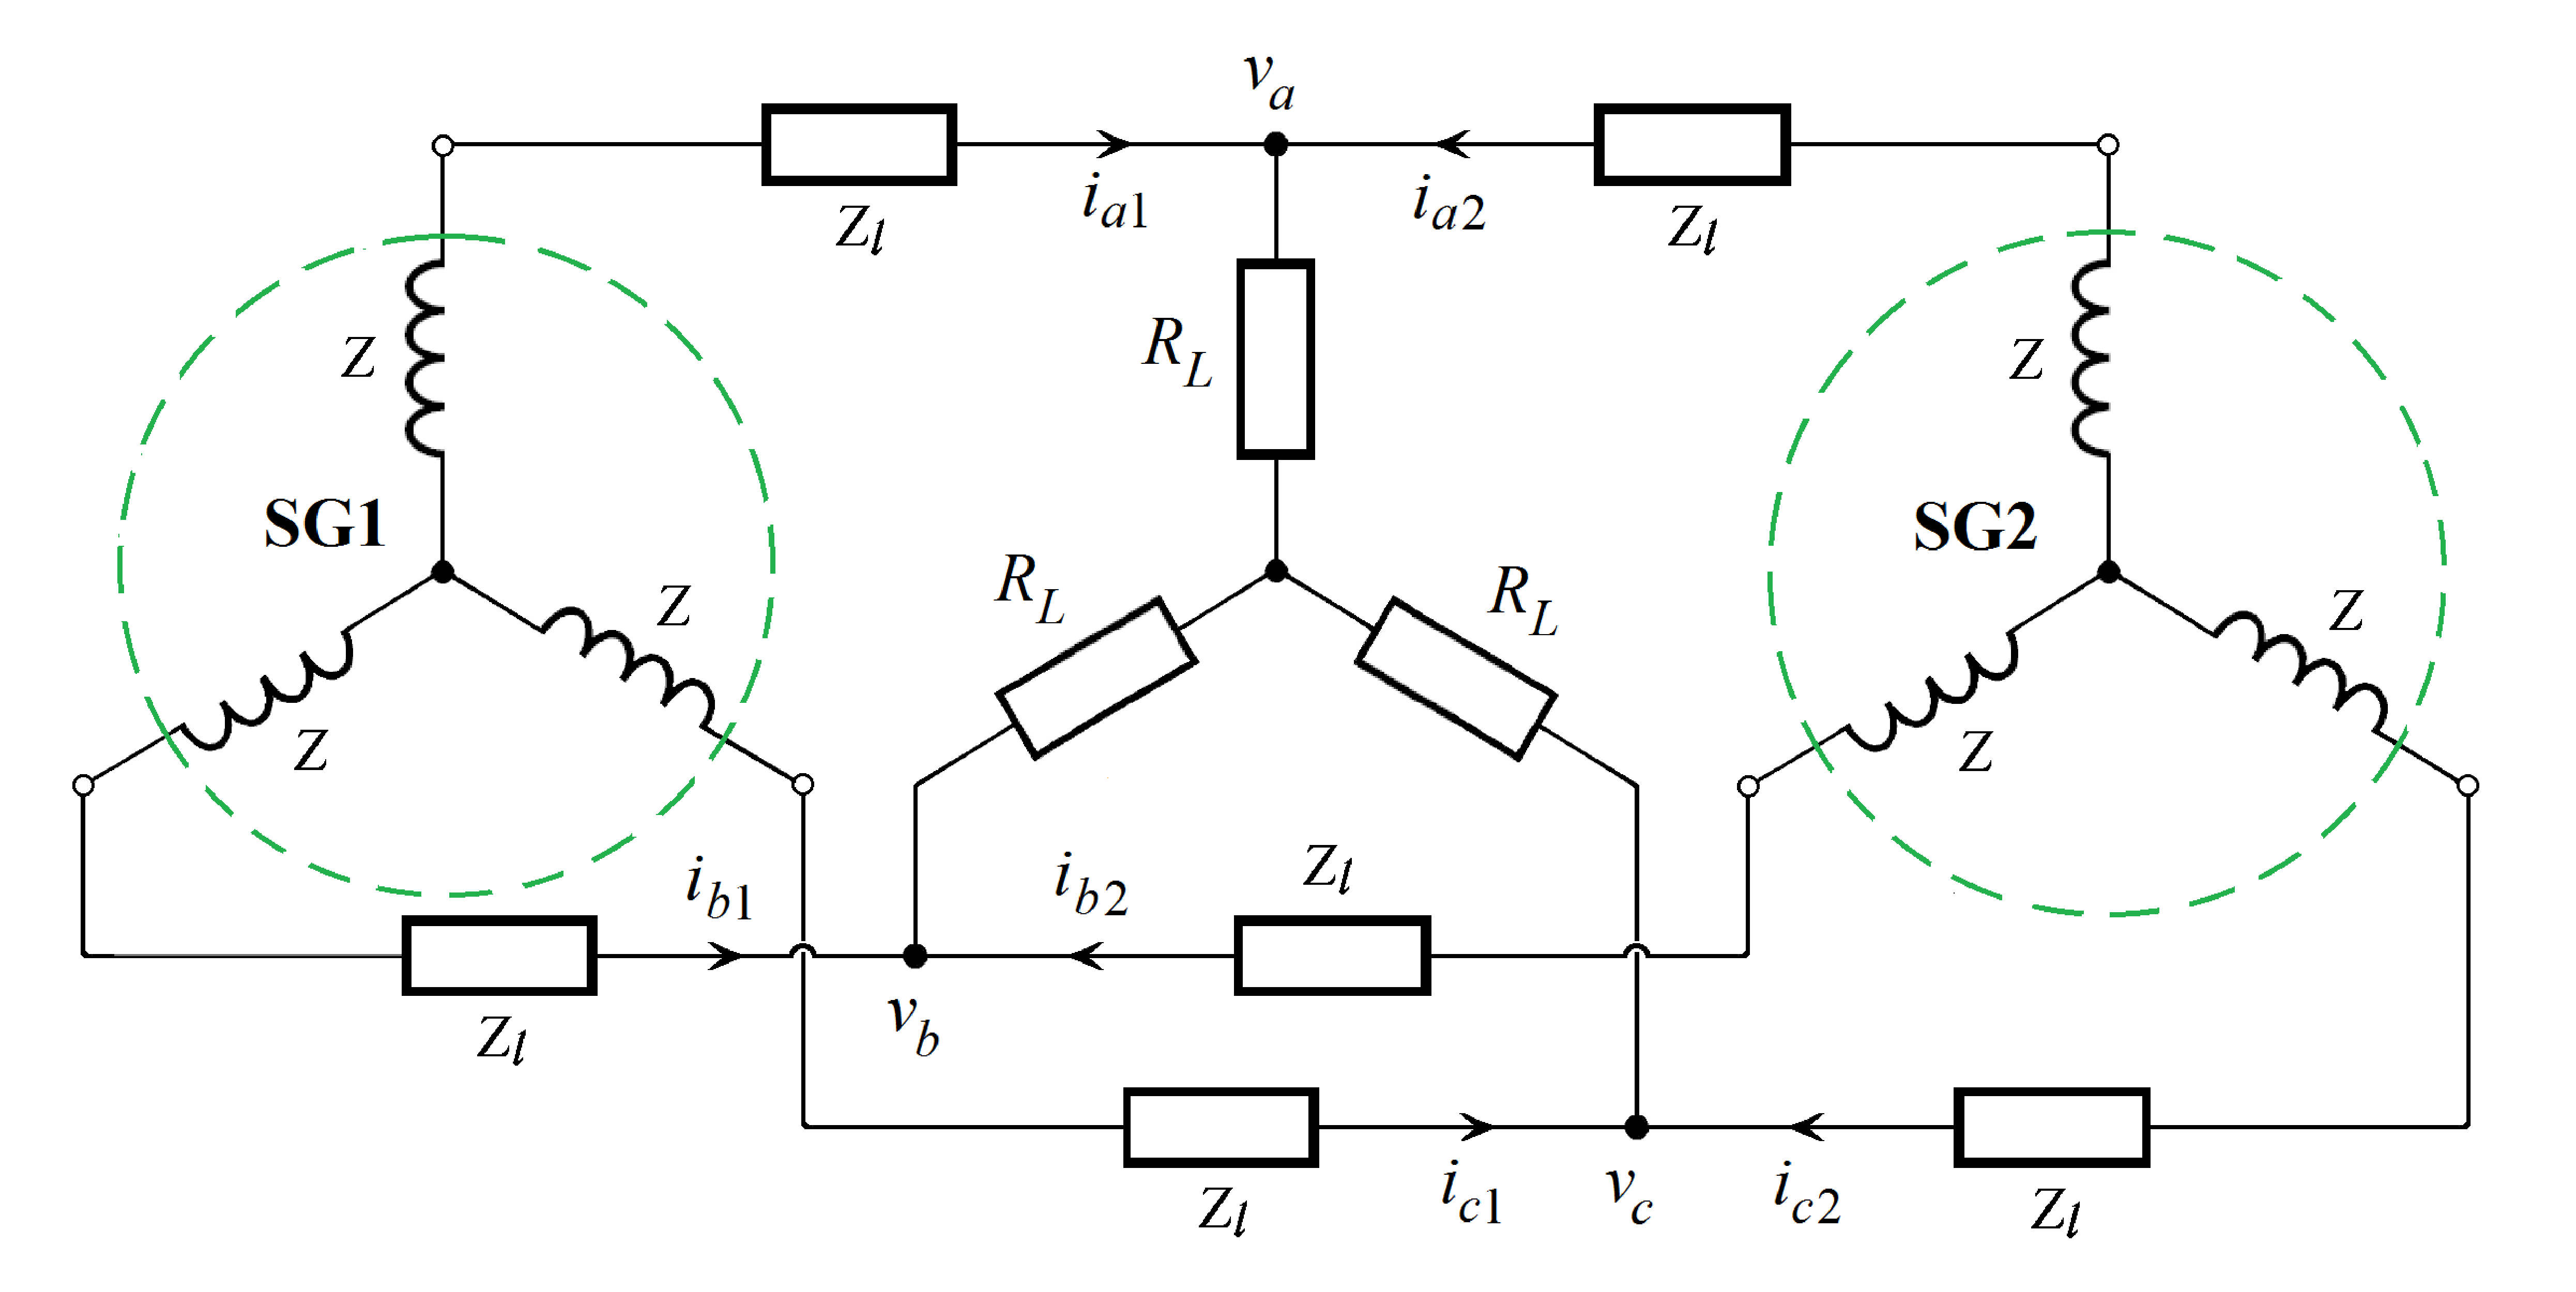
\includegraphics[width=8.5cm]{full_circuit_with_2_SGs}
\caption{The two identical coupled SGs (TICSG) model, showing the 
stator windings, the line impedances $Z_l$ and the load resistors 
$R_L$, but not showing the rotor windings or the prime movers.}
\label{fig:TICSGThreePhase}
\end{figure}
%%%%%%%%%%**********%%%%%%%%%%**********%%%%%%%%%%**********%%%%%%%%%%

The rest of this paper is organized as follows. In Section \ref{sec2}
a third order model of a SG having constant field current is
presented. The model of {\em two identical coupled SGs} (TICSG) is
described in Section \ref{sec3}. In Section \ref{sec4} we discuss the 
equilibrium points of the TICSG system. Stability analysis for the
TICSG model (in particular, results about the region of attraction of
the stable equilibrium point) is in Section \ref{sec5}. We illustrate
our results by simulations in Section \ref{sec6}. In particular, we 
show an example of two SGs where the region of attraction of the 
stable equilibrium point contains the submanifold where the 
generators have equal states (as it always does), but it does not 
contain all $\Xmscr$.

%%%%%%%%%%**********%%%%%%%%%%**********%%%%%%%%%%**********%%%%%%%%%%
\section{Modeling a single SG} \label{sec2} % Section 2

In this section we derive the equations for a SG connected to an
exernal voltage and having a constant field (or rotor) current,
following the notation in \cite{ZhWe:11}, see also \cite{NaWe:15}.

The rotor of a SG is a coil on a magnetic core that spins
inside a circular cavity in the stator, having the angle $\theta$ with
respect to a reference angle, see Figure 1. We denote its self
inductance by $L_f$, its resistance by $R_f$, the voltage across its
terminals by $v_f$ and the current through it (called the field
current) by $i_f$. We assume for simplicity that $L_f$ is independent
of $\theta$ and $i_f$. The stator consists of three identical windings
that are connected in a star, with phase shifts of $120^0$ (see again
Figure 1). We consider that there is no neutral connection and no
damper windings. The stator windings can be regarded as connected
coils with self inductance $L$, mutual inductance $-M$, and resistance
$R_s$ (the parameters $L_f,R_f,L,M,R_s$ are positive). We assume no
magnetic saturation effects in the iron core and no Eddy currents. The
stator terminals are labeled with the letters $a,b,c$ and the vector
of voltages on the stator terminals is denoted by $v=\left[v_a\ v_b\
v_c\right]^\top$. We denote by $v_s$ the voltage at the unconnected 
center of the star (see Figure 1) and $v^n=[v_s\ v_s\ v_s]^\top$.
We define the vectors
$$ \widetilde{\cos}\m\theta \m=\m \left[\begin{array}{c} \cos\left(
   \theta\right)\\ \cos\left(\theta-\frac{2\pi}{3}\right)\\
   \cos\left(\theta-\frac{4\pi}{3}\right) \end{array}\right] \m,\quad
   \widetilde{\sin}\m\theta \m= \left[\begin{array}{c} \sin\left(
   \theta\right)\\ \sin\left(\theta-\frac{2\pi}{3}\right)\\ \sin\left
   (\theta-\frac{4\pi}{3}\right) \end{array}\right] \m.$$
We denote the stator fluxes by $\Phi=\left[\Phi_a\ \Phi_b\ \Phi_c
\right]^\top$, the stator currents by $i=\left[i_a\ i_b\ i_c\right]
^\top$ and the rotor current by $i_f$. 

%%%%%%%%%%**********%%%%%%%%%%**********%%%%%%%%%%**********%%%%%%%%%%
\begin{figure} % Figure 2: single generator
\centering 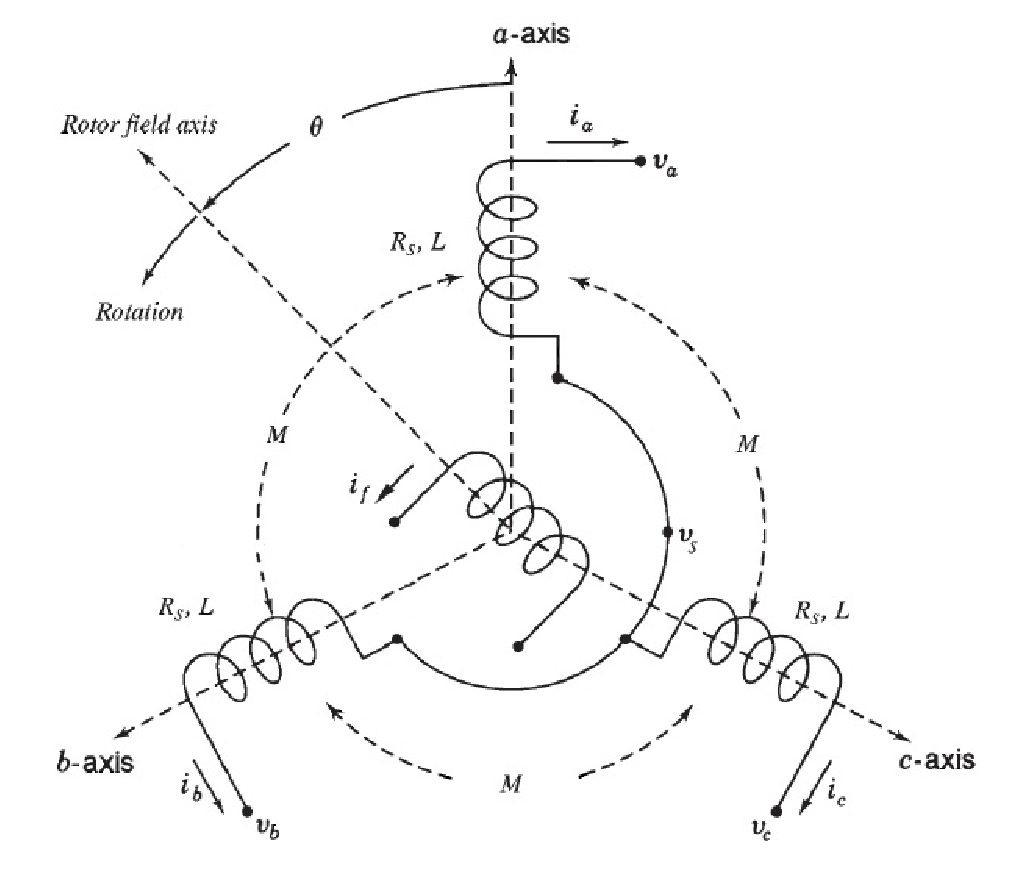
\includegraphics[width=7cm]{SGStructure.eps}
\caption[Structure of an idealized three-phase round rotor synchronous
generator]{Structure of an idealized three-phase round rotor
synchronous generator, modified from \cite[Figure 3.4]{GrSt2014}.}
\label{fig:structOfSG} \vspace{-3mm}
\end{figure}
%%%%%%%%%%**********%%%%%%%%%%**********%%%%%%%%%%**********%%%%%%%%%%

The mutual inductance between the rotor coil and each of the stator
coils varies with the rotor angle $\theta$ as follows:
$$ \left[\begin{array}{c} M_{a,f}\\ M_{b,f}\\ M_{c,f}\end{array}
   \right] \m=\m M_{f}\widetilde{\cos}\theta \m,$$
where $M_f>0$ is a constant. Hence, the vector of flux linkages of the
stator windings is
$$ \Phi \m=\m \left[\begin{array}{ccc} L & -M & -M\\ -M & L & -M\\
   -M & -M & L \end{array}\right]i + M_f i_f\widetilde{\cos}\theta
   \m.$$
Since there is no neutral line, $i_a+i_b+i_c=0$, so that the previous
equation can be rewritten as 
$$\Phi \m=\m L_s i + M_f i_f \widetilde{\cos}\theta \m,$$
where $L_s=L+M$. We will assume that the rotor current is constant
(or equivalently, the rotor is composed of a permanent magnet). The
stator voltages satisfy
\BEQ{eq:SGTerminalVlotage}
   v - v^n \m=\m -R_{s}i-\frac{\dd\Phi}{\dd t} \m=\m -R_{s}i-L_{s}
   \frac{\dd i}{\dd t} + e \m,
\end{equation}
where $e=\left[e_a\ e_b\ e_c \right] ^\top$ is the back electromotive 
force (EMF) due to the rotor movement (also called synchronous 
internal voltage), given by \vspace{-2mm}
\BEQ{eq:emf}
   e \m=\m M_f i_f\dot{\theta}\widetilde{\sin}\theta \m.
\end{equation}

For a SG with no load, the voltages at each terminal
will be sinusoidal functions. In order to represent the voltages and
currents in a more convenient way, we apply the Park transformation
with respect to the rotor angle:
$$ x_{dq0} \m=\m \left[\begin{array}{c} x_{d}\\ x_{q}\\ x_{0}
   \end{array}\right] \m=\m U(\theta) \left[\begin{array}{c} x_{a}\\
   x_b\\ x_c\end{array}\right] \m=\m U(\theta) x \m,$$
where $x$ is a vector in $abc$ coordinates, $x_{dq0}$
is the same vector in the $dq0$ coordinates, and $U(\theta)$ is the
following unitary matrix:
$$ U(\theta) \m=\m \sqrt{\frac{3}{2}}\left[\begin{array}{ccc}
   \cos(\theta) & \cos(\theta-\frac{2\pi}{3}) & \cos(\theta-
   \frac{4\pi}{3})\\ -\sin(\theta) & -\sin(\theta-\frac{2\pi}{3})
   & -\sin(\theta-\frac{4\pi}{3})\\ \sqrt{1/2} & \sqrt{1/2} & 
   \sqrt{1/2} \end{array}\right] \m.$$

Applying the Park transformation to \rfb{eq:SGTerminalVlotage} 
leads to
\BEQ{aPark}
   U(\theta)(v-v^n)-U(\theta)e \m=\m -R_{s}U(\theta)i - L_s 
   U(\theta) \frac{\dd i}{\dd t} \m.
\end{equation}
Now we use that, denoting $i_{dq0}=U(\theta)i$,
$$ \frac{\dd i_{dq0}}{\dd\theta} \m=\m U(\theta)\frac{\dd i}
   {\dd\theta} + \frac{\dd U(\theta)}{\dd\theta}i \m=\m
   U(\theta)\frac{\dd i}{\dd\theta} + \left[\begin{array}{c}
   i_{q}\\ -i_{d}\\ 0 \end{array}\right].$$
This implies that \vspace{-2mm}
$$ \dot{i}_{dq0} \m=\m \frac{\dd i_{dq0}}{\dd\theta} \cdot \frac
   {\dd\theta}{\dd t} \m=\m U(\theta)\dot{i} + \o\left[\begin{array}
   {c} i_q\\ -i_d\\ 0 \end{array}\right] \m,$$
where 
$$\o=\dot{\theta}.$$
 We rewrite \rfb{aPark} as follows:
\BEQ{eq:idiqDynamics}
   L_s\frac{\dd}{\dd t}\nm\left[\nm\begin{array}{c} i_d\\ i_q\\ i_0
   \end{array}\nm\right] - L_s \o \left[\nm\begin{array}{c} i_q\\ -i_d
   \\ 0 \end{array}\nm\right] = -R_s\left[\begin{array}{c} i_d\\
   i_q\\ i_0 \end{array}\right] + \left[\nm \begin{array}{c} e_d-v_d
   \\ e_q-v_q\\ \tilde v\end{array}\nm\right],
\end{equation}
where $\tilde v=e_0-v_0+v^n_0$. Here we have used that (obviously)
$v^n_d=v^n_q=0$. Since there is no neutral connection, $i_0=0$, hence
$\tilde v=0$. Applying the Park transformation to \rfb{eq:emf} gives
$$ \left[\begin{array}{c} e_d\\ e_q \end{array}\right] \m=\m -\sqrt
   {\frac{3}{2}} M_{f} \left[ \begin{array}{c} 0\\ \o i_f
   \end{array}\right] \m.$$
We denote 
$$m=\sqrt{\frac{3}{2}}M_{f}.$$ If we substitute the last
formula into \rfb{eq:idiqDynamics}, we get
\BEQ{eq:idiqDynamicsWithExIf}
   L_s\frac{\dd}{\dd t} \nm \left[\nm \begin{array}{c}
   i_d\\ i_q \end{array} \nm\right] = -R_s\left[\nm \begin{array}{c}
   i_d\\ i_q \end{array} \nm\right]+\o L_s\left[\nm\nm \begin{array}
   {c} i_q\\ -i_d\end{array} \nm\nm\right]\\ -m\left[\nm\nm 
   \begin{array}{c} 0\\ \o i_f\end{array} \nm\nm\right] - \left[\nm 
   \begin{array}{c} v_d\\ v_q \end{array} \nm\right] .
\end{equation}

The rotational dynamics of the rotor is given by
\BEQ{eq:mechanicalPart}
   J\dot{\omega} \m=\m T_{m}-T_{e}-D_{p} \omega \m,
\end{equation}
where $J$ is the moment of inertia of the rotor, $T_m-D_p\o$ is is the
mechanical torque coming from the prime mover, $T_e$ is the
electromagnetic torque developed by the generator, and $D_p$ is a the
frequency droop coefficient employed in the prime movers connected to
the generators. If any viscous friction is present, it can be absorbed
into the term $D_p\o$. All the parameters $J,T_m,D_p$ are positive.
The feedback term $D_p\o$ is used in order to control the frequency of
the grid, see \cite{Kundur}, \cite{PoDoBu:13}, \cite{CaTa:14},
\cite{ZhWe:11}. $T_e$ can be found using energy consideration. The 
magnetic energy stored in the generator is
$$ E_{mag} \m=\m \half \left(\langle i,L_s i \rangle + L_f i_f^2
   \right) + M_f i_f \langle i,\widetilde{\cos}\theta \rangle \m.$$
The electromagnetic torque can be calculated as follows:
$$ T_e \m=\m \frac{\partial E_{mag}}{\partial\theta}|_{\Phi,\Phi_f
   \ const.} \m=\m - \frac{\partial E_{mag}}{\partial\theta}|_{i,
   i_f\ const.}$$
(see \cite{ZhWe:11}), whence
$$ T_e \m=\m M_f i_f \left\langle i,\frac{\dd\tilde{\cos}\theta}
   {\dd\theta} \right\rangle \m=\m M_f i_f \langle i,\widetilde
   {\sin} \theta\rangle \m=\m -m i_f i_q \m.$$
Using \rfb{eq:idiqDynamicsWithExIf}, \rfb{eq:mechanicalPart}
and the last formula, we obtain
\BEQ{eq:SingleSGDynamics}
   \frac{\dd}{\dd t}\nm\left[\nm \begin{array}{c} L_s i_d\\ L_s i_q\\ 
   J\o\end{array} \nm\right] = \left[\nm \begin{array}{ccc} -R_s & 
   \o L_s & 0\\ -\o L_s & -R_s & -mi_f\\ 0 & mi_f & -D_p \end{array}
   \nm\right] \nm \left[\nm \begin{array}{c} i_d\\ i_q\\ \o 
   \end{array} \nm\right] + \left[\nm\nm \begin{array}{c} -v_d\\ -v_q
   \\ T_m \end{array} \nm\nm\right].
\end{equation}
This third order nonlinear dynamical system represents the dynamics of
a single SG with constant field current, if we ignore the dynamics of
the rotor angle $\theta$.

%%%%%%%%%%**********%%%%%%%%%%**********%%%%%%%%%%**********%%%%%%%%%%
\section{TICSG modeling} \label{sec3} % Section 3

In this section we develop the TICSG model that represent two 
identical SGs connected to a common resistive load, as shown in
Figure \ref{fig:TICSGThreePhase}, assuming constant field currents.
The model of each SG is as in Section \ref{sec2}.

We denote the SG rotor angles by $\theta_1$ and $\theta_2$ and
$\o_1=\dot\theta_1$, $\o_2=\dot\theta_2$. We assume that identical
prime movers act on the generators, producing the torques
$T_{m}-D_p\o_i$, $i\in\{1,2\}$. By symmetry, we assume that the
voltages at the (non-connected) midpoints of the generators and the
load are zero. We denoted the phase voltages on the load by
$v=\left[v_a\ v_b\ v_c \right]^\top$, the currents of the first
generator by $i_1=\left[i_{a1} \ i_{b1}\ i_{c1}\right]^\top$ and 
similarly for the currents of the second generator.
%by $i_2=\left[i_{a2}\ i_{b2}\ i_{c2}\right]^\top$.

In Figure \ref{fig:TICSGThreePhase} we have indicated by $Z$ the
equivalent impedance of each SG stator, $Z=sL_s+R_s$. The line that
connects the SG to the load has its impedance $Z_l$ that can be
modeled as a resistance and an inductance in series, but these values
can simply be added to the parameters $R_s$ and $L_s$ of the SG. After
this simplification, each phase of the circuit from Figure
\ref{fig:TICSGThreePhase} is as in Figure \ref{fig:TICSGOnePhase}.

%%%%%%%%%%**********%%%%%%%%%%**********%%%%%%%%%%**********%%%%%%%%%%
\begin{figure} % Figure 3: Tree phase TICSG system
\centering 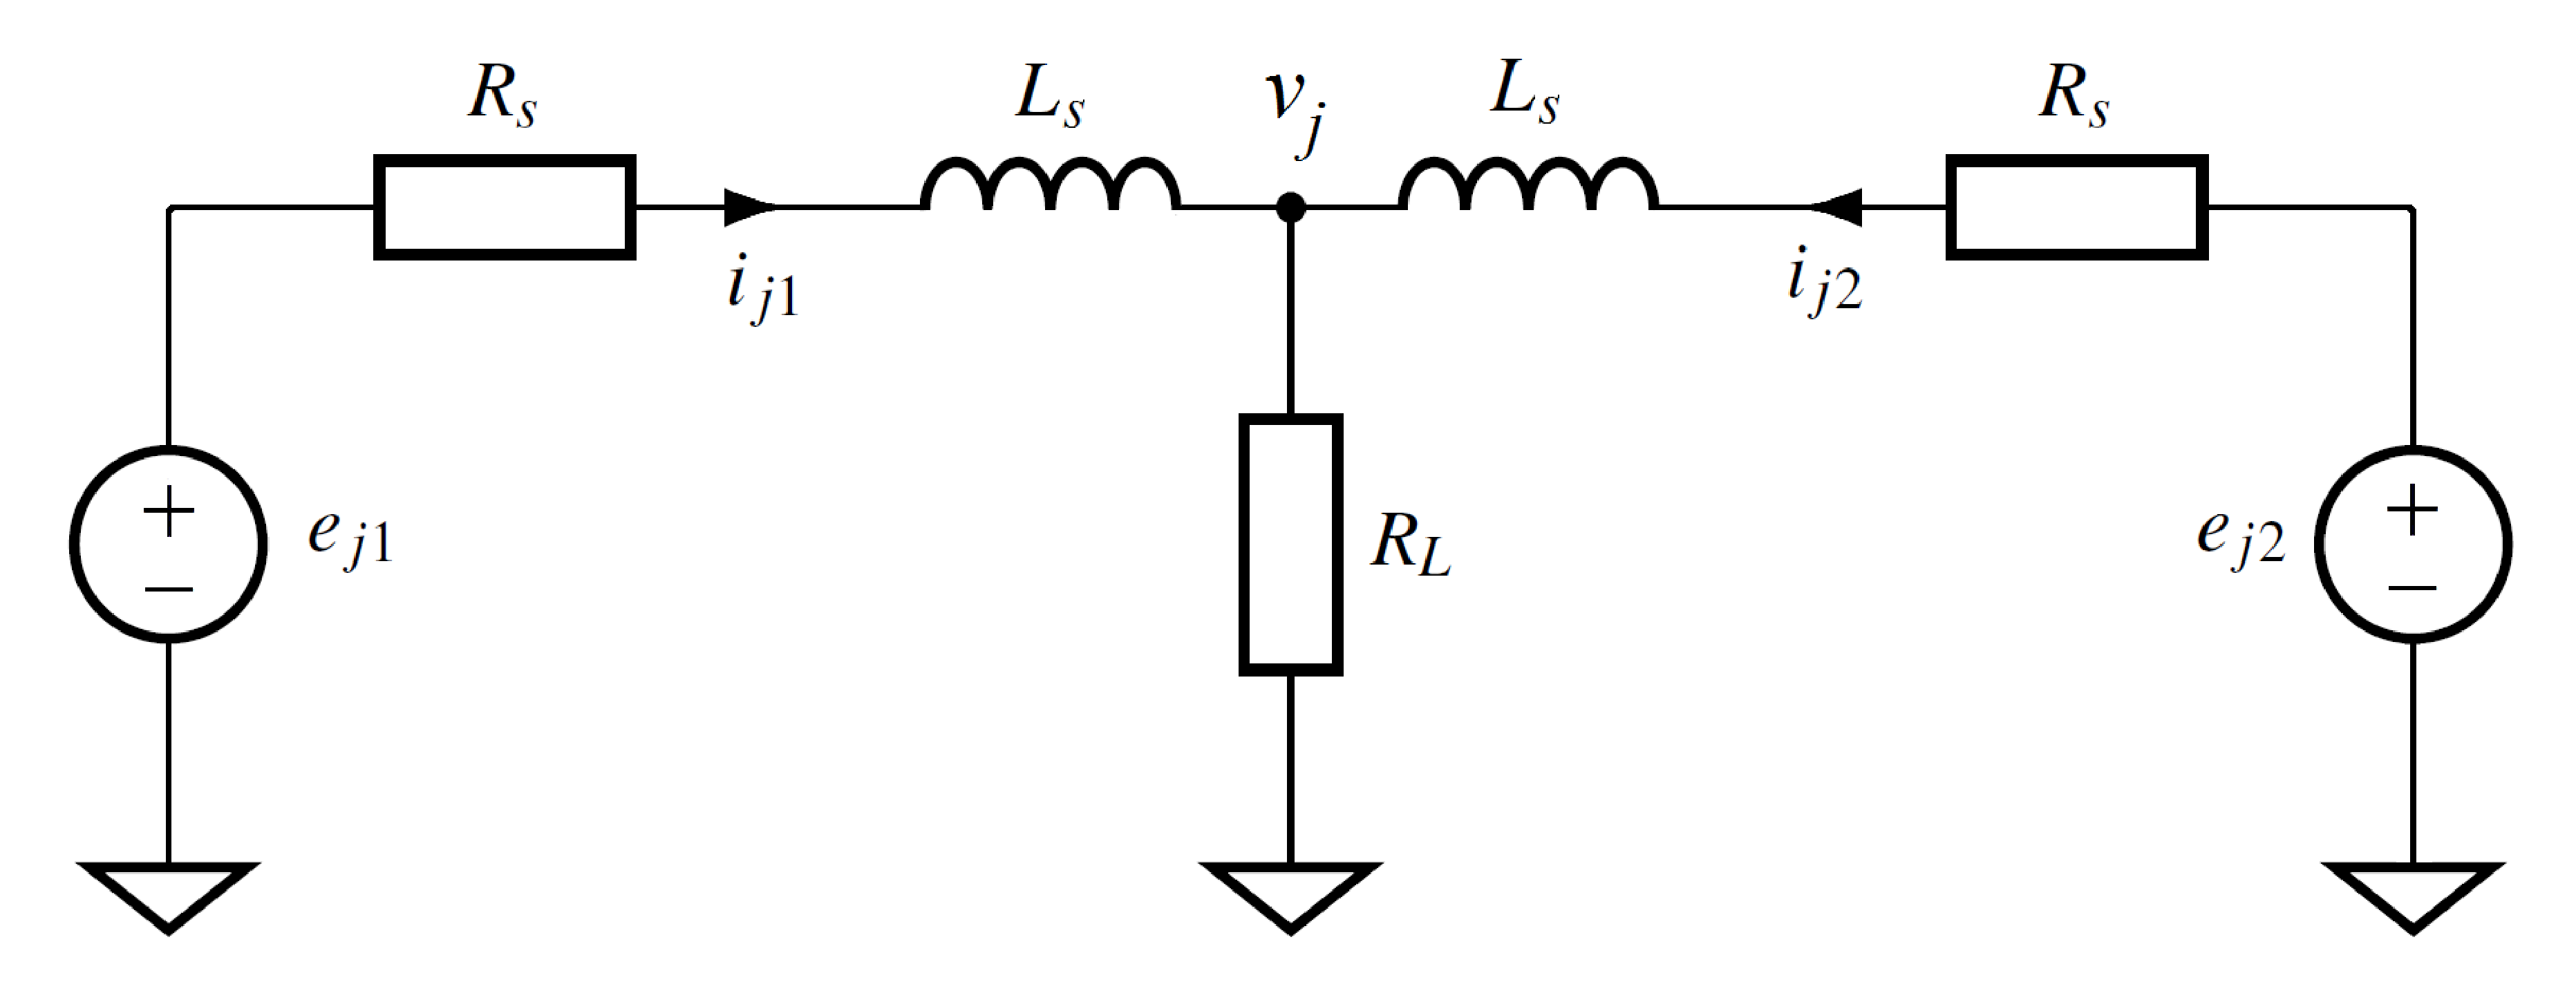
\includegraphics[width=8cm]{one_phase.eps}
\vspace{-3mm}
\caption{The TICSG model - equivalent circuit for one phase, 
$j\in\{a,b,c\}.$} \vspace{-6mm}
\label{fig:TICSGOnePhase}
\end{figure}
%%%%%%%%%%**********%%%%%%%%%%**********%%%%%%%%%%**********%%%%%%%%%%

In order to use the model \eqref{eq:SingleSGDynamics} for each SG, we
apply the Park transformation (defined in the previous section) to the
load voltages, $\left[ v_{d1}\ v_{q1}\ v_{01}\right]^\top=U(\theta_1)
\left[v_a\ v_b\ v_c\right] ^\top$, and to the currents $\left[i_{d1}\
i_{q1}\ i_{01} \right]^\top=U(\theta_1)\left[i_{a1}\ i_{b1}\
i_{c1}\right]^\top$, and similarly for $i_2$ and $\theta_2$. From
$v=R_L(i_1+i_2)$ we get, after applying the Park transformation with
respect to $\theta_1$,
$$ \left[\begin{array}{c} v_{d1}\\ v_{q1}\\ v_{01} \end{array}
   \right] \m=\m R_L\left[\begin{array}{c} i_{d1}\\ i_{q1}\\
   i_{01} \end{array}\right] + R_L U(\theta_1)\left[\begin{array}{c}
   i_{a2}\\ i_{b2}\\ i_{c2} \end{array}\right] \m.$$
Here we express the currents of the second SG by using the inverse 
Park transformation: 
\BEQ{eq:TICSGVolAndCurr}
   \left[\begin{array}{c} v_{d1}\\ v_{q1}\\ v_{01} \end{array}\right]
   \m=\m R_{L}\left[\begin{array}{c} i_{d1}\\ i_{q1}\\ i_{01}
   \end{array}\right] + R_L U(\theta_1)U(\theta_2)^{-1}\left[
   \begin{array}{c} i_{d2}\\ i_{q2}\\ i_{02} \end{array}\right].
\end{equation}

We denote \vspace{-3mm}
$$\delta \m=\m \theta_2 - \theta_1 \m.$$
A simple computation shows that 
\BEQ{eq:ParkChangeAngle}
   U(\theta_{1})U(\theta_{2})^{-1}=\left[\begin{array}{ccc}
   \cos(\delta) & -\sin(\delta) & 0\\ \sin(\delta) & \cos(\delta) 
   & 0\\ 0 & 0 & 1 \end{array}\right].
\end{equation}
Since the SGs don't have a neutral connection, from Kirchhoff's
laws we obtain that $i_{01}=i_{02}=0$. Substituting this into
\eqref{eq:TICSGVolAndCurr} and \eqref{eq:ParkChangeAngle} shows that
$v_{01}=0$.

Substituting \eqref{eq:ParkChangeAngle} and \eqref{eq:TICSGVolAndCurr}
into \eqref{eq:SingleSGDynamics} gives:
$$ \varLambda\dot{z}_1 \m=\m \mathcal{A}(\o_1)z_1+T_m e_3 - 
   \mathcal{B}(\delta)z_2 \m,$$
where we have denoted
$$ z_i \m=\m \left[i_{di}\ i_{qi}\ \o_i\right]^\top,\quad 
   i\in\{1,2\},$$
$$ \varLambda \m=\m \left[\begin{array}{ccc} L_s & 0 & 0\\
   0 & L_{s} & 0\\ 0 & 0 & J \end{array}\right],$$
$$ \mathcal{A}(\o) \m=\m \left[\begin{array}{ccc}
   -R_{tot} & \o L_s & 0\\ -\o L_s & -R_{tot} & -mi_{f}\\
   0 & mi_{f} & -D_{p} \end{array}\right],$$
$$ \mathcal{B}(\delta) \m=\m \left[\begin{array}{ccc}
   R_L\cos(\delta) & -R_{L}\sin(\delta) & 0\\ R_L\sin(\delta) & 
   R_L\cos(\delta) & 0\\ 0 & 0 & 0 \end{array}\right],$$
$$e_{3}=\left[0\ 0\ 1\right]^\top, \quad  R_{tot}=R_{s}+R_{L}.$$
A symmetric equation holds for the second generator:
$$ \varLambda\dot{z}_2 \m=\m \mathcal{A}(\o_{2})z_{2}+T_{m}e_{3} -
   \mathcal{B}(-\delta)z_{1} \m.$$
An additional ODE for $\delta$ is:
$$\dot{\delta} \m=\m \o_2-\o_1 \m.$$

Rewriting the entire TICSG system dynamics gives:
\begin{equation} \label{eq:TICSGDynamics}
   \frac{\dd}{\dd t}\left[\nm\nm\begin{array}{c} \varLambda z_{1}\\
   \varLambda z_{2}\\ \delta \end{array}\nm\nm\right] = \left[\nm
   \nm\begin{array}{c|c|c} \mathcal{A}(\o_1) & -\mathcal{B}(\delta)
   & 0\\ -\mathcal{B}(-\delta) & \mathcal{A}(\o_2) & 0\\ -e_{3}^T
   & e_3^T & 0 \end{array}\nm\right] \left[\nm\begin{array}{c} z_1
   \\ z_2\\ \delta \end{array}\nm\right] + T_m \left[\nm 
   \begin{array}{c} e_{3}\\ e_{3}\\ 0 \end{array} \nm\right].
\end{equation}

\begin{lemma}\label{lemma:forewordComplete}
The TICSG system is forward complete, i.e. for any initial state
$\left[ z_1^{0\top} \ z_2^{0\top} \ \delta^{0} \right]^\top \in
\mathbb{R}^7 $, the (unique) solution of the TICSG system is defined
for all $t>0$.
\end{lemma}

\begin{proof} The right hand-side of the TICSG model 
\eqref{eq:TICSGDynamics} is a locally Lipschitz function on the state
space $\rline^7$. For any initial state it follows from standard well
posedness results (see for instance \cite[Ch.~3]{Khalil}) that there
exists a unique solution $(z_1,z_2,\delta)$ for
\eqref{eq:TICSGDynamics} defined on a maximal time interval
$[0,{T_{\max}})$, with ${T_{\max}}>0$. We will show via contradiction that
${T_{\max}}=\infty$. Suppose that $T_{\max}$ is finite. For each $t\in
[0,{T_{\max}})$ define
$$ V\left(\left[\nm\begin{array}{c} z_1\\ z_2\end{array}\nm\right]
   \right) \m=\m \half \left[z_1^\top\ z_2^\top\right]\left[
   \begin{array}{cc} \varLambda & 0\\ 0 & \varLambda \end{array}
   \right]\left[ \begin{array}{c} z_1\\ z_2 \end{array}\right].$$
Then, using \eqref{eq:TICSGDynamics},
$$ \dot{V}(t) \m=\m \left[ z_1^\top\ z_2^\top\right]\left[\nm
   \begin{array}{cc} \varLambda & 0\\ 0 & \varLambda \end{array}
   \nm\right]\left[\begin{array}{c} \dot{z_1}\\ \dot{z_2}
   \end{array}\right]$$ 
$$ = \left[z_1^\top\ z_2^\top\right]\left[\nm\nm
   \begin{array}{cc} \varLambda & 0\\ 0 & \varLambda \end{array}
   \nm\nm\right] \left[\nm\nm\begin{array}{c} \varLambda^{-1}
   \left( \Amscr(\o_1)z_1-\Bmscr(\delta)z_2+T_me_3\right)
   \\ \varLambda^{-1}\left(-\mathcal{B}(-\delta)z_1+\mathcal{A}
   (\o_2)z_2+T_m e_3\right) \end{array}\nm\right].$$
Because $\mathcal{B}(-\delta) = \mathcal{B}^\top(\delta)$, we get 
$$ \begin{aligned} \dot{V}(t) =& \left(z_1^\top\mathcal{A}(\o_1)
   z_1+z_2^\top\mathcal{A}(\o_2)z_2\right) \\ &+ \left(-2z_1^\top
   \mathcal{B}(\delta)z_2 + T_mz_1^\top e_3+ T_mz_2^\top e_3\right)
   \end{aligned}$$
$$ \begin{aligned} =& \left(-R_{tot}\left(i_{d1}^2 +
   i_{q1}^2+i_{d2}^2+i_{q2}^2 \right)-D_p \left(\o_1^2+\o_2^2\right)
   \right) \\ & +2 R_L \left(-\cos(\delta)i_{d1}i_{d2}-\cos(\delta)
   i_{q1}i_{q2}-\sin(\delta)i_{q1}i_{d2}\right)\\ &+2 R_L
   \sin(\delta)i_{q2}i_{d1} + T_m(\o_1+\o_2).\end{aligned}$$
This equation can be rewritten as
$$ \dot{V}(t) \m=\m -D_p\left( \o_1^2+\o_2^2\right) + T_m(\o_1+\o_2)
   -\langle A\vec{i},\vec{i} \rangle \m,$$ 
where $\vec{i}=[i_{d1}\ i_{q1}\ i_{d2}\ i_{q2}]^\top$ and 
$$ \begin{aligned} A &=\left[\begin{array}{cc|cc} R_{tot} & 0 & R_L 
   \cos(\delta) & -R_L \sin(\delta) \\ 0 & R_{tot} & R_L R_L 
   \sin(\delta) & R_L\cos(\delta) \\ \hline R_L\cos(\delta) & R_L 
   \sin(\delta) & R_{tot} & 0 \\ -R_L \sin(\delta) & R_L\cos(\delta) 
   & 0 & R_{tot} \end{array}\right]\\ &= \left[ \begin{array}{c|c}
   A_1 & B \\ \hline B^* & A_1 \end{array} \right].\end{aligned}$$

According to the well known Schur complement condition for positive
definiteness, a symmetric matrix $X = \left[ \begin{array}{c|c} P_1 &
N \\ \hline N^* & P_2 \end{array}\right]$ is positive definite if and
only if $P_1>0$ and $\Delta=P_2-N^*P_1^{-1}N>0$. In our case clearly
$A_1>0$. Thus, in order to show that $A>0$ we only need to show that 
$A_1-B^*A_1^{-1}B>0$. By a simple computation,
$$ A_1-B^*A_1^{-1}B \m=\m \left[\begin{array}{cc}
   R_{tot}-\frac{R_L^2}{R_{tot}} & 0  \\ 
   0 & R_{tot}-\frac{R_L^2}{R_{tot}} \end{array}\right].$$
Since $R_{tot}>R_L$, we have indeed $A_1-B^*A_1^{-1}B>0$. 

From $A>0$, if either $|i_{d1}|$, $|i_{q1}|$, $|\o_1|$, $|i_{d2}|$,
$|i_{q2}|$ or $|\o_2|$ is sufficiently large, then
$\dot{V}(t)<0$. Therefore $V$ (and hence $i_{d1}$, $i_{q1}$, $\o_1$,
$i_{d2}$, $i_{q2}$ and $\o_2$ are bounded on $[0,{T_{\max}})$. Clearly
$\delta$ must also be bounded on $[0,{T_{\max}})$. Hence $(i_{d1},
i_{q1},\o_1,i_{d2},i_{q2},\o_2)$ are bounded on $[0,{T_{\max}})$, which
contradicts \cite[Corollary II.3]{JayWeissBS:09}. Therefore 
${T_{\max}}=\infty$.
\end{proof}
 
%%%%%%%%%%**********%%%%%%%%%%**********%%%%%%%%%%**********%%%%%%%%%%
\section{Analysis of the equilibrium points of the TICSG model} 
\label{sec4} % Section 4

In this section we study the equilibrium points of the TICSG
system \eqref{eq:TICSGDynamics}. We introduce the {\em synchronization 
subspace} of the state space $\rline^7$ by
\begin{equation} \label{eq:SyncSubspace}
   \Emscr \m=\m \left\{ \left[z_1 \ z_2 \ \delta \right]^\top\in
   \rline^7 \ |\ z_1=z_2,\ \delta = 0 \right\} \m.
\end{equation}
Clearly this is a 3-dimensional vector subspace. Similarly, we
introduce the {\em anti-synchronization space}
\begin{equation} \label{eq:AntiSyncSubspace}
   \Emscr' \m=\m \left\{ \left[z_1 \ z_2 \ \delta \right]^\top
   \ |\ z_1=z_2,\ \delta = \pi \right\} \m,
\end{equation}
which is an affine space (shifted vector subspace). Sometimes we find
it more convenient to consider the angle $\delta$ modulo $2\pi$, so
that the seventh coordinate of the state is no longer in $\rline$, but
instead in the unit circle. This new state space $\Xmscr$ is a 7
dimensional manifold, with a natural mapping from $\rline^7$ to
$\Xmscr$ (which leaves the first 6 coordinates unchanged), and the
images of $\Emscr$ and $\Emscr'$ via this mapping are 3 dimensional
submanifolds of $\Xmscr$ that we denote by $\Emscr_\Xmscr$ and
$\Emscr'_\Xmscr$, respectively. We call $\Emscr_\Xmscr$ the 
{\em symchronization manifold}.

\begin{proposition} \label{EqPointsProp1}
Any equilibrium point for the TICS system in $\Xmscr$ is either in
$\Emscr_\Xmscr$ or in $\Emscr'_\Xmscr$.
\end{proposition}

\begin{proof}
The equilibrium points are the solutions of the algebraic equation
\begin{equation} \label{eq:algebricEquation}
   \left[\nm\begin{array}{c|c|c} \Amscr(\o_1^e) & -\Bmscr(\delta^e) &
   0\\ \hline -\Bmscr(-\delta^e) & \Amscr(\o_2^e) & 0\\ \hline -e_3^T 
   & e_3^T & 0\end{array} \nm\right] \left[\nm\begin{array}{c} z_1^e
   \\ z_2^e\\ \delta^e\end{array}\nm\right] + T_m\left[\nm
   \begin{array}{c} e_{3}\\ e_{3}\\ 0 \end{array}\nm\right] = 0.
\end{equation}
It easy to see that according to the seventh line above,
$$\o_1^e \m=\m \o_2^e \m=\m \o^e \m.$$
From the third and the sixth lines we have: 
$$ \left\{ \begin{array}{c} m i_f i_{q1}^e-D_p\o_1^e+T_m=0\\
   mi_f i_{q2}^e-D_p\o_2^e+T_m=0 \end{array}\right.\Longrightarrow
   i_{q1}^{e}=i_{q2}^{e}=i_{q}^{e} \m.$$
From the first, second, fourth and fifth lines:
$$ \begin{array}{c} -R_{tot}i_{d1}^e+\o^e L_s i_q^e-R_L\cos\delta^e
   i_{d2}^e+R_L\sin\delta^e i_q^e=0,\\ -\o^e L_s i_{d1}^e-R_{tot} 
   i_q^e-mi_f\o^e-R_L\sin\delta^e i_{d2}^e-R_L\cos\delta^e i_q^e=0,\\
   -R_{tot}i_{d2}^e+\o^e L_s i_q^e-R_L\cos\delta^e i_{d1}^e-R_L
   \sin\delta^e i_q^e=0,\\ -\o^e L_s i_{d2}^e-R_{tot}i_q^e-mi_f
   \o^e+R_L\sin\delta^e i_{d1}^e-R_L\cos\delta^e i_q^e=0.\end{array}$$
By denoting \vspace{-2mm}
$$ M \m=\m \left[\begin{array}{cc} -R_{tot} & -R_{L}\cos\delta^{e}\\
   -\o^e L_s & -R_L\sin\delta^e\\ -R_L\cos\delta^e & -R_{tot}\\
   R_L\sin\delta^e & -\o^e L_s \end{array}\right]$$
and 
$$ n \m=\m \left[\begin{array}{c} i_q^e\left(\o^e L_s+R_L\sin\delta^e
   \right)\\ -mi_f\o^e-i_q^e\left(R_{tot}+R_L\cos\delta^e\right)\\
   i_q^e\left(\o^e L_s-R_L\sin\delta^e\right)\\ -mi_f\o^e-i_q^e\left(
   R_{tot}+R_L\cos\delta^e\right) \end{array}\right]$$
we rewrite these lines in the following way:
\begin{equation} \label{eq:equilibrium_system}
   M\left[\begin{array}{c} i_{d1}^e\\ i_{d2}^e \end{array}\right]
   \m=\m n \m.
\end{equation}

Now, we show by contradiction that any equilibrium point must satisfy
$\sin\delta^e=0$. We use the Rouch\'e Capelli theorem: Any liner
equations system with the form $Mx=n$ has a solution if and only if
rank$\left[M|n\right]=$rank$\left[M\right]$. If we would have
$\sin\delta^e\neq 0$, then a simple calculation shows that 
rank$\left[M|n\right]=3$ must hold.

Obviously, rank$\left[M\right]\leq 2$. The Rouch\'e Capelli theorem
implies that under the previous assumption the linear equations system
\eqref{eq:equilibrium_system} does not have any solution. It proves
that if the TICSG system has an equilibrium point, it must satisfy
$\sin\delta^{e}=0$, whence $\delta^{e}=0$ or $\delta^e=\pi$
(modulo $2\pi$).

After substituting $\sin\delta^{e}=0$ and $\cos\delta^{e}=\pm 1$, the 
matrices in the equation \eqref{eq:equilibrium_system} become
$$ M \m=\m \left[\begin{array}{cc} -R_{tot} & \mp R_L\\ -\o^e L_s & 
   0\\ \mp R_L & -R_{tot}\\ 0 & -\o^e L_s \end{array}\right] \m,$$
$$ n \m=\m \left[\begin{array}{c} i_q^e\o^e L_s\\ -mi_f\o^e-i_q^e
   \left(R_{tot} \pm R_L\right)\\ i_q^e\o^e L_s\\ -mi_f\o^e-i_q^e
   \left(R_{tot} \pm R_L\right) \end{array}\right] \m.$$
Now the only solution of \eqref{eq:equilibrium_system} is
$i_{d1}^{e}=i_{d2}^{e}$.
\end{proof}

\begin{proposition} \label{EqPointsProp2}
The TICSG system has at least one equilibrium point on
synchronization subspace $\Emscr$ from \eqref{eq:SyncSubspace}.
\end{proposition}

\begin{proof}
For a point in $\Emscr$ we obtain from \eqref{eq:SyncSubspace} that
\begin{equation} \label{eq:equilbrium_algebric_eq}
   \left[\nm\nm\begin{array}{ccc} -R_s-2R_L & \o^e L_s & 0\\
   -\o^e L_s & -R_s-2R_L & -m i_f\\ 0 & m i_f & -D_p
   \end{array} \nm\right] \left[\nm\begin{array}{c} i_d^e\\
   i_q^e\\ \o^e \end{array} \nm\right] = \left[\nm\nm 
   \begin{array}{c} 0\\ 0\\ -T_m\end{array} \nm\nm\right]\nm\m,
\end{equation}
where $i_d^e,i_q^e,\o^e$ are the coordinates of $z_1^e=z_2^e=z^e$.
From \eqref{eq:equilbrium_algebric_eq} we derive a scalar equation to
determine the equilibrium velocity $\omega^{e}$. From the last line of
the equation we have
\begin{equation} \label{eq:eq_0_first_eq}
   T_m-D_p\o^e \m=\m -mi_f i_q^e 
\end{equation}
The left side of this equation is the mechanical torque acting on each
generator at equilibrium.

The first line of \eqref{eq:equilbrium_algebric_eq}
is $-\left(R_{tot}+R_L\right)i_d^e+\o^e L_{tot}i_q^e=0$, \quad hence
$$i_d^e \m=\m \frac{\o^e L_s}{R_{tot}+R_L} i_q^e \m.$$
From \eqref{eq:eq_0_first_eq} we have
$$i_q^e \m=\m \frac{T_m-D_p\o^e}{-mi_f} \m.$$
Combining the last two formulas,
$$ i_{d}^{e} \m=\m -\frac{\o^e L_s}{R_{tot}+R_L} \cdot \frac{T_m-D_p
   \o^e}{mi_f} \m.$$

The second line of the matrix equation on \eqref{eq:eq_0_first_eq} is
$$ \o^{e}L_s i_d^e + \left(R_{tot} + R_L\right) i_q^e + mi_f\o^e 
   \m=\m 0 \m.$$
Substituting in this equation the expressions for $i_q^e$ and
$i_d^e$ yields the following cubic equation in $\o^e$, where
we denote $R_T=R_L+R_{tot}$:
\begin{equation}
 D_p L_s^2\o^{e3}-T_m L_s^2 \o^{e2} +\left(D_p R_T^2+m^2 i_f^2 
   R_T\right) \o^e - T_m R_T^2 \m=\m 0 \m.
\label{eq:cubicEqation}   
\end{equation}

Let us denote the polynomial of order 3 appearing above by $p$. 
Clearly \vspace{-2mm}
$$p(0) \m=\m -T_m R_T^2 \m<\m 0 \m.$$
On the other hand, we note that 
$$ p\left(\frac{T_m}{D_p}\right) \m=\m m^2 i_f^2 R_T\frac{T_m}{D_p} 
   \m>\m 0 \m.$$
Hence, $p$ has at least one zero in the interval $\left(0,
\frac{T_m}{D_p}\right)$. This shows that the TICSG system has at least
one equilibrium point located on the synchronization subspace 
\eqref{eq:SyncSubspace}.
\end{proof}

Note that $\Emscr'_\Xmscr$ may also contain equilibrium points.

\begin{remark}
If we take scalar products on both sides of 
\eqref{eq:equilbrium_algebric_eq} with $z^e$, we obtain
$$ \left(R_{tot}+R_L\right)\left((i_d^e)^2+(i_q^e)^2\right) \m=\m
   \left(T_m-D_p\o^e\right)\o^e \m.$$
This equation makes perfect physical sense. Indeed, assume that there
is no actual friction in the machine, $D_{p}$ is created by feedback,
so that $T_{m}-D_{p}\omega^{e}$ is the mechanical torque applied to
one generator, and then $\left(T_{m}-D_{p}\omega^{e}\right)\omega^{e}$
is the mechanical power entering one generator. On the other hand, it
is easy to see that $\left(R_{tot}+R_L\right)\left((i_d^e)^2+
(i_q^e)^2\right)=\left(R_s+2R_L\right)\left(i_a^2+i_b^2+i_c^2\right)$
which is exactly half of the power dissipated in all the resistors,
hence it is the electric power leaving one generator.
\end{remark}

%%%%%%%%%%**********%%%%%%%%%%**********%%%%%%%%%%**********%%%%%%%%%%
\section{Synchronization} \label{sec5} % Section 5

In this section, we show that the synchronization subspace
$\mathscr{E}$ from \eqref{eq:SyncSubspace} is invariant and locally
exponentially stable for the TICSG model \eqref{eq:TICSGDynamics}.  We
start by rewriting the TICSG model in new coordinates. Then, we prove
that under some conditions, the TICSG is globally exponentially stable
in the subspce $\mathscr{E}$. Finally, we use the main result from
\cite{AndrieuJayawardhanaPraly}, to show the stability of the system
near the synchronization subspace.

%%%%%%%%%%**********%%%%%%%%%%**********%%%%%%%%%%**********%%%%%%%%%%
\subsection{Modeling the synchronization problem:} 
\label{sec:SyncProbModel}

The TICSG system has the following structure:
$$ \tilde{\Lambda}\frac{d}{dt}\left[z_1\ z_2\ \delta\right]^{\top}
   \m=\m f\left( \left[z_1\ z_2\ \delta\right]^{\top} \right) \m,$$
where $\tilde{\Lambda}={\rm diag}\left(\Lambda,\Lambda,1\right)$.
In order to show synchronization, it is convenient to introduce new 
state variables $e\in\rline^4$ and $x\in\rline^3$ by
$$ e \m=\m \left[ \begin{array}{c} z_2 - z_1\\ \delta \end{array} 
   \right] \m=\m \left[e_d\ e_q\ e_\o\ \delta \right]^\top$$
and 
$$x =z_1+z_2 = \left[ x_d\ x_q\ x_\omega\right]^\top.$$  

Then the TICSG model \eqref{eq:TICSGDynamics} can be rewritten as

\begin{equation}
\dot{e}=F(e,x) , \quad \dot{x}=G(e,x),\label{eq:sync_sestem}
\end{equation}
for some functions $F$ and $G$. From \eqref{eq:TICSGDynamics},
$$ \begin{aligned} \Lambda(\dot{z}_2-\dot{z}_1) &= \Amscr(\o_2)
   z_2+T_m e_3-\Bmscr(-\delta)z_1\\ &-\left(\Amscr(\o_1)z_1+T_m 
   e_3-\Bmscr(\delta)z_2\right) \end{aligned} \m.$$
The detailed form of the equation $\dot e=F(e,x)$ is
$$ \begin{aligned} & \left[\begin{array}{cc} \varLambda & 0\\ 0 & 
   1 \end{array}\right] \frac{\dd}{\dd t}\left[\begin{array}{c}
   e_d\\ e_q\\ e_\o\\ \delta\end{array}\right] \m= \\ & \left[\nm
   \begin{array}{c} -R_{tot}(i_{d2}-i_{d1})+L_s(\o_2 i_{q2}-
   \o_1 i_{q1})\\ -L_s(\o_2 i_{d2}-\o_1 i_{d1})-R_{tot} (i_{q2}
   -i_{q1})-mi_f(\o_2-\o_1)\\ mi_f(i_{q2}-i_{q1})-D_p(\o_2-\o_1)
   \\ -(\o_2-\o_1) \end{array}\nm\right]\\ + & \left[\begin{array}
   {c} R_L\cos(\delta)(i_{d2}-i_{d1})-R_L\sin(\delta)(i_{q2}
   +i_{q1})\\ R_L\cos(\delta)(i_{q2}-i_{q1})+R_L\sin(\delta)(i_{d2}
   +i_{d1})\\ 0\\ 0 \end{array}\right]. \end{aligned}$$
From the trivial identity \m $(a+b)(x-y)+(a-b)(x+y)=2(ax-by)$ we
get that \vspace{-2mm}
$$ \begin{aligned} \o_2 i_{q2} -& \o_1 i_{q1} \m=\m \half\left[
   (\o_1+\o_1)(i_{q2}-i_{q1}) \right.\\ &+ \left. (\o_2-\o_1)(i_{q2}
   +i_{q1})\right] = \frac{x_{w} e_q+e_w x_q}{2} \end{aligned}$$
and the previous equation can be rewritten as:
$$ \dot{e} \m=\m F(e,x) \m=\m \left[\nm\begin{array}{cc} \varLambda 
   & 0\\ 0 & 1 \end{array}\nm\right]^{-1} \left[A_e\left(x,e\right) 
   e + B_e \left(x,e\right) \right]$$
where 
$$ \begin{aligned}
&A_e\left(x,e\right)  = \\ & \left[\begin{array}{cccc}
-R_{tot}+R_{L}\cos\delta & \frac{L_{s}}{2}x_{\omega} & \frac{L_{s}}{2}x_{q} & 0\\
-\frac{L_{s}}{2}x_{\omega} & -R_{tot}+R_{L}\cos\delta & -\frac{L_{s}}{2}x_{d}-mi_f & 0\\
0 & mi_{f} & -D_{p} & 0\\
0 & 0 & 1 & 0
\end{array}\right]
\end{aligned}
$$ 
and
$$
B_e\left(x,e\right) = 
\left[\begin{array}{c}
-R_{L}\sin(\delta)x_{q}\\
R_{L}\sin(\delta)x_{d}\\
0\\
0
\end{array}\right].
$$

Note that the synchronization subspace $\mathscr{E}$ from \eqref{eq:SyncSubspace}, in the new coordinates, becomes $\mathscr{E}=\left\{\left[ \begin{array}{c}
x \\
e
\end{array}\right] \in\mathbb{R}^{7}|e=0 \right\}$.
We note that $F(0,x)=0$, which shows that 
$\mathscr{E} $ is invariant.

For the $x$ dynamics we have
$$ \begin{aligned} \Lambda\dot{x} \m=\m & \Amscr(\o_1) z_1 + T_m e_3
   -\Bmscr(\delta) z_2\\ +& \Amscr(\o_2) z_2 + T_m e_3-\Bmscr
   (-\delta) z_1, \end{aligned}$$
$$ \begin{aligned} &\Lambda\frac{\dd}{\dd t}\left[\begin{array}{c}
   x_{d}\\ x_{q}\\ x_{\o} \end{array}\right] = \\
   & \left[\begin{array}{c} - R_{tot}(i_{d1}+i_{d2})+L_s(\o_1 i_{q1}
   +\o_2 i_{q2})\\ -L_s(\o_1 i_{d1}+\o_2 i_{d2})-R_{tot}(i_{q1} +
   i_{q2})-m i_f(\o_1+\o_2)\\ m i_f(i_{q1}+i_{q2})-D_p(\o_1+\o_2) +
   2T_m \end{array}\right]\\ +& \left[ \begin{array}{c}
   -R_L\cos(\delta)(i_{d1}+i_{d2})-R_L\sin(\delta)(i_{q1}-i_{q2})\\
   -R_L\cos(\delta)(i_{q1}+i_{q2})+R_L\sin(\delta)(i_{d1}-i_{d2})\\
   0 \end{array}\right] \end{aligned}$$

From the trivial identity $(a+b)(x+y)+(a-b)(x-y)=2(ax+by)$ it 
follows that
$$ \begin{aligned} \o_1 i_{q1}+\o_2 i_{q2} &= \half\left[(\o_1+\o_2)
   (i_{q1}+i_{q2})+(\o_1-\o_2)(i_{q1}-i_{q2})\right]\\ & =\frac{x_{w}
   x_{q}+e_{w}e_{q}}{2} \end{aligned} $$
and similarly \vspace{-3mm}
$$ \o_1 i_{d1}-\o_2 i_{d2} \m=\m \frac{x_{w}x_{d}+e_{w}e_d}{2} \m.$$

The $x$ dynamics can be rewritten as:
$$ \dot{x}=G \left( x,e\right) \m=\m \Lambda^{-1}\left(A_x \left(x,e 
   \right) x + B_x \left( x,e\right) \right),$$
where
$$ A_x \left(x,e \right) = \left[\nm\nm\begin{array}{ccc}
   -R_{tot}-R_L\cos(\delta) & \frac{L_s}{2} x_\o & 0\\
   -\frac{L_s}{2} x_\o & -R_{tot}-R_L\cos(\delta) & -mi_f\\
   0 & mi_f & -D_p\end{array} \nm\right]$$
$$ B_x \left(x,e \right)=\left[\begin{array}{c}
   \frac{L_{s}}{2}e_{\omega}e_{q}-R_{L}\sin(\delta)e_{q}\\
   -\frac{L_{s}}{2}e_{\omega}e_{d}-R_{L}\sin(\delta)e_{d}\\
   2T_{m} \end{array}\right] \m.$$

%%%%%%%%%%**********%%%%%%%%%%**********%%%%%%%%%%**********%%%%%%%%%%
\subsection{Global exponential stability of the TICSG system on the
synchronization subspace }

In this subsection, we provide sufficient conditions for the
equilibrium point which located on the synchronization subspace
$\mathscr{E}=\left\{ \left[ e\ x \right]^\top\in\mathbb{R}^{7}|e=0
\right\}$ to be a globally exponential stable equilibrium point, for
trajectories with initial condition that lies in $\mathscr{E}$.
(Recall that $\mathscr{E}$ is an invariant subspace.)

We denote the state variables of this system by $\tilde{x}=
\left[x_d\ x_q\ x_\o\right]^\top$. The dynamics of these trajectories
is (denoted as $\tilde{G}$):
$$ \dot{\tilde{x}} \m=\m \tilde{G}(\tilde{x}) = G(0,\tilde{x}) =
   \Lambda^{-1} A\left( \tilde{x}_\omega \right) \tilde{x}+
   \Lambda^{-1} B \m,$$
where we denote
$$ A\left( \tilde{x}_\o \right) \m=\m A_x\left(0, \tilde{x}_\o
   \right) \m=\m \left[\begin{array}{ccc} - R_T & \frac{L_s}{2}
   \tilde{x}_\o & 0\\ -\frac{L_{s}}{2}\tilde{x}_\o & -R_T & -mi_f\\
   0 & mi_{f} & -D_{p} \end{array}\right]$$
and
$$ B \m=\m B_x\left(0, \tilde{x}_\o \right) \m=\m \left[\begin{array}
   {c} 0\\ 0\\ 2T_m \end{array}\right].$$
This system describes the two SGs with perfect synchronization between
each other.

Because the TICSG system has at least one equilibrium point on
$\Emscr$, it means that $\tilde{G}(\tilde{x})$ has at least one
equilibrium point $\tilde{x}^{e}=\left[\tilde{x}_{d}^{e}\
\tilde{x}_{q}^{e}\ \tilde{x}_{\omega}^{e} \right]^\top = 2z^e$ (recall
that by definition $x = z_1 + z_2$). We have
\begin{equation}
\tilde{G}(\tilde{x}^{e})=0\rightarrow\varLambda^{-1}A(\tilde{x}_{\omega}^{e})\tilde{x}^{e}+\varLambda^{-1}\left[\begin{array}{c}
0\\
0\\
2T_{m}
\end{array}\right]=0\label{eq:G_at_equilibrium}
\end{equation}

In order to shift the equilibrium point into the origin, we introduce the new  coordinates
$$
\hat{x}\coloneqq\tilde{x}-\tilde{x}^{e}
$$

A natural Lyapunov function candidate for this system is 
$$
V(\hat{x})\coloneqq\frac{1}{2}L_{s}\left(\hat{x}_{d}^{2}+\hat{x}_{q}^{2}\right)+\frac{1}{2}J\tilde{\omega}^{2}=\frac{1}{2}\hat{x}^{T}\varLambda\hat{x}.
$$

It is easy to see that:
$$
\frac{1}{2} min\left\{L_{s},J\right\}|\hat{x}|{}^{2}\leq V(\hat{x})\leq \frac{1}{2} max\left\{L_{s},J\right\}|\hat{x}|{}^{2}
$$

$$
\left|\frac{\partial V}{\partial\hat{x}}\right|=\left|\varLambda\hat{x}\right|\leq max\left\{L_{s},J\right\}\left|\hat{x}\right|
$$

We calculate $\dot{V}(\hat{x})$ in order to show that under some
conditions, $\dot{V}(\hat{x})\leq\alpha|\hat{x}|{}^{2}$, for some
$\alpha$. This proves that $\tilde{G}(\tilde{x})$ is globally
exponentially stable (see for instance Theorum 5.17, p.~195 in
\cite{Sastry}).

$$
\dot{V}(\hat{x})=\left(\frac{\partial V}{\partial\hat{x}}\right)^{T}\dot{\hat{x}}
$$

\begin{equation}
\dot{\hat{x}}=\dot{\tilde{x}}=\varLambda^{-1}A(\tilde{x}_\omega)\tilde{x}+\varLambda^{-1}\left[\begin{array}{c}
0\\
0\\
2T_{m}
\end{array}\right]\label{eq:x_hat_dynamic}
\end{equation}
 
We rewrite  $A(\tilde{x}_{\omega})$ as a sum of a constant symmetric
matrix, constant skew symmetric matrix and a skew symmetric matrix
which depends on $\hat{x}_{\omega}$:
$$ 
A(\tilde{x}_{\omega})\tilde{x}=\left[R+J(\tilde{x}_{\omega}^{e})+\Delta(\hat{x}_{\omega})\right](\hat{x}+\tilde{x}^{e}) \m,
$$
where
$$ R \m=\m \left[\begin{array}{ccc} -R_T & 0 & 0\\
   0 & -R_T & 0\\ 0 & 0 & -D_{p}
\end{array}\right] \m,$$
$$ J \m=\m \left[\begin{array}{ccc} 0 & \frac{L_s}{2}\tilde{\o}^e
   & 0\\ -\frac{L_s}{2}\tilde{\o}^e & 0 & -mi_f\\ 0 & mi_f & 0
   \end{array}\right] \m,$$
$$ \Delta(\hat{x}_\o)\coloneqq\left[\begin{array}{ccc}
   0 & \frac{L_{s}}{2}\hat{x}_{\omega} & 0\\
   -\frac{L_{s}}{2}\hat{x}_\o & 0 & 0\\
   0 & 0 & 0 \end{array}\right] \m.$$
Combining the previous equation with \eqref{eq:G_at_equilibrium} and
\eqref{eq:x_hat_dynamic} gives
$$ \dot{\hat{x}}=\Lambda^{-1}\left( \left[R+J+\Delta(\hat{\o})
   \right]\hat{x}+\Delta(\hat{\o})\tilde{x}^{e}\right) \m.$$

We calculate the derivative of $V$ over time: 
$$ \dot{V}(\hat{x}) \m=\m \left(\L\hat{x}\right)^T\dot{\hat{x}}
   \m=\m \hat{x}^T\L^T\L^{-1}\left( \left[R+J+\Delta(\hat{x}_\o)
   \right]\hat{x}+\Delta(\hat{x}_{\omega})\tilde{x}^{e}\right).$$
Because $\L$ is a diagonal matrix, $\L^T\L^{-1}=I$. Thus, 
$$ \dot{V}(\hat{x}) \m=\m \hat{x}^{T}R\hat{x}+\hat{x}^T J\hat{x}
   +\hat{x}^T\Delta(\hat{x}_\o)\hat{x}+\hat{x}^T\Delta(\hat{x}_\o)
   \tilde{x}^e \m.$$
Because $J(\tilde{\o}^e)$ and $\Delta(\hat{\o})$ are 
skew-symmetric matrices, $\hat{x}^{T}J(\tilde{\o}^e)\hat{x}=0$
and $\hat{x}^T\Delta(\hat{\o})\hat{x}=0$. We have
$$ \begin{aligned} \hat{x}^{T}\Delta(\hat{x}_\o)\tilde{x}^{e} 
   \m=\m &\left[\begin{array}{c} \hat{x}_d\\ \hat{x}_q\\ \hat{x}_\o
   \end{array}\right]^T\left[\begin{array}{ccc} 0 & \frac{L_s}{2}
   \hat{x}_\o & 0\\ -\frac{L_s}{2}\hat{x}_\o & 0 & 0\\ 0 & 0 & 0
   \end{array}\right]\left[\begin{array}{c} x_d^e\\ x_q^e\\
   \tilde{x}_\o^e \end{array}\right]\\ =& \left[\begin{array}{c}
   \hat{x}_d\\ \hat{x}_q\\ \hat{x}_\o \end{array}\right]^T\left[\nm
   \begin{array}{ccc} 0 & 0 & \frac{L_s}{4}x_q^e\\ 0 & 0 & 
   -\frac{L_s}{4}x_d^e\\ \frac{L_s}{4}x_q^e & -\frac{L_s}{4}x_d^e
   & 0 \end{array}\nm\right] \left[\nm\begin{array}{c} \hat{x}_d\\
   \hat{x}_q\\ \hat{x}_\o \end{array}\nm\right] \\ =\m & 
   \hat{x}^{\top} P\hat{x} \m,\end{aligned}$$
where we have denoted
$$ P \m=\m \left[\begin{array}{ccc} 0 & 0 & \frac{L_{s}}{4}
   x_{q}^{e}\\ 0 & 0 & -\frac{L_s}{4} x_d^e\\ \frac{L_s}{4} x_q^e 
   & -\frac{L_s}{4} x_d^e & 0 \end{array}\right] \m.$$
Combining all this together, we obtain 
$$\dot{V}(\hat{x}) \m=\m \hat{x}^{T}\left[P+R\right]\hat{x} \m,$$
where 
$$ P+R \m=\m \left[\begin{array}{ccc} -R_T & 0 & \frac{L_s}{4}
   x_q^e\\ 0 & -R_T & -\frac{L_s}{4} x_d^e\\ \frac{L_s}{4} x_q^e 
   & -\frac{L_s}{4} x_d^e & -D_p \end{array}\right].$$
Calculating the eigenvalues of $P+R$ gives \m $\l_{1}=-R_T<0$,
$$ \l_{2,3} \m=\m -\frac{R_T+D_p}{2} \pm\frac{\sqrt{4\left(R_T-D_p
   \right)^2+L_s^2\left(\left(x_q^e\right)^2 + \left(x_d^e
   \right)^2\right)}}{4} \m.$$
All the eigenvalues are real. The condition which guarantees that
all the three eigenvalues are negative is:
\begin{equation} \label{eq:condition_for_stable_G}
   16 R_T D_p \m>\m L_s^2 \left( \left(x_q^e\right)^2+\left( x_d^e
   \right)^2\right) \m.
\end{equation}
When condition \eqref{eq:condition_for_stable_G} holds, then
$\dot{V}(\hat{x})<-min\left(\left|\lambda_{i}\right|\right)|
\hat{x}|^{2},\quad i\in\{1,2,3\}$, and this system is globally
exponentially stable. Note that because it proves global stability in
$\mathscr{E}$, it means that $\tilde{x}^{e}$ is the only equilibrium
point of $\dot{\tilde{x}}=\tilde{G}(\tilde{x})$, hence the TICSG
system has exactly one equilibrium point on the the synchronization
subspace $\Emscr$.

%%%%%%%%%%**********%%%%%%%%%%**********%%%%%%%%%%**********%%%%%%%%%%
\subsection{Synchronization theorem:}
 
In this subsection, we prove that if the initial state of the two
generators are sufficiently close to each other, i.e $|e(0)|$ is small
enough, then, under some conditions, the two generators will
synchronize, meaning that $\lim_{t\to\infty}e(t)=0$.

In order to show that, we use the main result of 
\cite{AndrieuJayawardhanaPraly}. Consider a system of the form 
\begin{equation} \label{eq:systemForm}
   \dot{e} \m=\m F\left(e,x\right),\quad \dot{x} \m=\m
   G\left(e,x\right) \m,
\end{equation}
where $e$ and $x$ are finite-dimensional real vector valued functions
and $F, G \in C^2$ with $F(0,x)=0$. \cite{AndrieuJayawardhanaPraly}
defines the following properties:

\subsubsection{TULES-NL (transversal uniform local exponential 
stability)} There exist positive numbers $r$, $k$ and $\l$ such that
we have, for all $\left(e_0, x_0, t\right)$ where $\left| e_0\right|
\le r$ and the solution satisfies $\left|e\left(e_0, x_0,
t\right)\right| \le k\left|e_0\right| e^{-\l t}$. Namely the
manifold $\mathscr{E}$ is exponentially stable locally in $e$,
uniformly in $x$.
\subsubsection{UES-TL (uniform exponential stability for the 
transversally linear system)} There exist strictly positive real 
numbers $\tilde{k}$ and $\tilde{\l}$ such that any solution $\left(e 
\left(e_0,x_0,t\right),x\left(x_0, t\right)\right)$ of the 
transversally linear system
$$ \dot{\tilde{e}} \m=\m \frac{\partial F(e,x)}{\partial e}
   \left(0,\tilde{x}\right),\quad\ \dot{\tilde{x}} \m=\m \tilde{G}
   \left(\tilde{x}\right) \m=\m G\left(0,x\right)$$
satisfies, for all initial states $e_0$ and $x_0$ and for all $t>0$,
$$ \left| \tilde{e}\right(\tilde{e}_0,\tilde{x}_0,t \left) \right| 
   \m\leq\m \tilde{k} e^{-\l t} \left| \tilde{e}_0\right| \m.$$ 
In other words, the manifold $\tilde{\Emscr}=\left\{\left(\tilde{e},
\tilde{x} \right)| \tilde{e} = 0 \right\}$ is exponentially stable 
for this system, uniformly in $\tilde{x}$.

\begin{theorem}\label{therem:TULESNL2UESTL}
If a  system  has form \eqref{eq:systemForm}, and it forward complete, and it satisfies the following conditions in an invariant  compact sets that contains the initial conditions : 
\begin{enumerate}
\item 
There exist a positive real number $\mu$, such that: 
$$
\left|\frac{\partial F(e,x)}{\partial e}(0,x)\right| \le \mu. 
$$
\label{condition1}
\item 
The manifold $\mathscr{E}$ is invariant.
\label{condition2}
\item
If there exist positive definite matrix $Q$, such the function $P:\mathbb{R}^{n_x}\to\mathbb{R}^{n_e \times n_e}$ given by
$$P\left(\tilde{x}\right)=\lim_{T \to+\infty} \int_0^T \left( \frac{\partial \tilde{E}}{\partial \tilde{e}}\left(0,\tilde{x},s\right)\right)^\top Q \frac{\partial \tilde{E}}{\partial \tilde{e}}\left(0,\tilde{x},s\right) ds$$
exist (\cite{AndrieuJayawardhanaPraly} sows that $P$ always exist for UES-TL systems that satisfies conditions 1 and 2).
 \label{condition3}
\item 
there exist positive real numbers $\eta$ and $c$ such that, for all $(e,x)$ in $B_e(\eta)\times \mathbb{R}^n_x$,
$$\left| \frac{\partial P}{\partial x}(x)\right| \le c,$$
$$\quad  \left| \frac{\partial^2 F}{\partial e \partial e}(e,x)\right| \le c, \quad  \left| \frac{\partial^2 F}{\partial x \partial e}(e,x)\right| \le c,\quad\left| \frac{\partial G}{\partial e}(e,x)\right| \le c$$
\label{condition4}
\end{enumerate}
then the UES-TL property implies the TULES-NL property for this system.
\end{theorem}

This theorem is one of the main results of \cite{AndrieuJayawardhanaPraly}. See \cite[Comment 2, p.3]{AndrieuJayawardhanaPraly}.

Now, we use this theorem in order to show that the TICSG has the TULES-NL property.

We start with calculating $\frac{\partial F(e,x)}{\partial e}(0,x)$. We can express $F$ as composed of two functions $F_\zeta$ and $F_\delta$:
$$
\begin{aligned}
 F = \left[\begin{array}{cc} F_\zeta \\ F_\delta \end{array}\right] &= \left[\begin{array}{cc}
\varLambda & 0\\
0 & 1
\end{array}\right]^{-1} \left[\begin{array}{cc}
A_{e_z}(x,\delta) & 0\\
e_3^\top & 0
\end{array}\right]   \left[\begin{array}{cc} e_\zeta \\ \delta \end{array}\right]    \\ &+ \left[\begin{array}{cc}
\varLambda & 0\\
0 & 1
\end{array}\right]^{-1}B_e\left(x,\delta\right)
\end{aligned}
$$
where $A_e(x,\delta) = \left[\begin{array}{cc}
A_{e_z}(x,\delta) & 0\\
e_3^\top & 0
\end{array}\right] $ and $e_\zeta = \left[e_d \ e_q \ e_\omega \right]^\top$.

$$
\frac{\partial F(e,x)}{\partial e}(0,x)=\left[\begin{array}{cccc}
 \frac{\partial F_\zeta}{\partial e_\zeta} & \frac{\partial F_\zeta}{\partial \delta} \\
\frac{\partial F_\delta}{\partial e_\zeta}  & \frac{\partial F_\delta}{\partial \delta}

\end{array}\right].
$$
We have 
$$
\begin{aligned}
&\frac{\partial F_\zeta}{\partial e_\zeta}(0,x)=\varLambda^{-1}A_{e_z}(x,0) \\&=\left[\begin{array}{ccc}
-R_{tot}+R_{L} & \frac{L_{s}}{2}x_{\omega} & \frac{L_{s}}{2}x_{q} \\
-\frac{L_{s}}{2}x_{\omega} & -R_{tot}+R_{L} & -\frac{L_{s}}{2}x_{d}-mi_f \\
0 & mi_{f} & -D_{p} 
\end{array}\right],
\end{aligned}
$$

$$
\begin{aligned}
 \frac{\partial F_\zeta}{\partial \delta} & =  \varLambda^{-1} \frac{\partial F_\zeta}{\partial \delta}\left( A_{e_\zeta}(x,\delta) \right)e_\zeta+ \frac{\partial F_\zeta}{\partial \delta}\left(B_e(x,\delta)\right)
 \end{aligned}
$$
$$
 \frac{\partial F_\zeta}{\partial \delta}(0,x)  =  \left[\begin{array}{ccc}
 -R_L x_q\\
R_Lx_d\\
0
\end{array}\right],\quad \frac{\partial F_\delta}{\partial e_\zeta}=e_3^\top,\quad \frac{\partial F_\delta}{\partial \delta}
=0$$
Finally
\begin{equation}
\frac{\partial F(e,x)}{\partial e}(0,x)=\left[\begin{array}{cccc}
-\frac{R_{s}}{L_{s}} & \frac{x_{\omega}}{2} & \frac{x_{q}}{2} & -\frac{R_{L}}{L_{s}}x_{q}\\
-\frac{x_{\omega}}{2} & -\frac{R_{s}}{L_{s}} & -\frac{x_{d}}{2}-\frac{mi_f}{L_{s}} & \frac{R_{L}}{L_{s}}x_{d}\\
0 & \frac{mi_{f}}{J} & -\frac{D_{p}}{J} & 0\\
0 & 0 & 1 & 0
\end{array}\right]
\label{eq:AOft}
\end{equation}

\begin{theorem}\label{theorem:TICSGSync}
If TICSG system satisfies condition \eqref{eq:condition_for_stable_G},
and in addition
\begin{equation} \label{eq:eLinearizationLimit}
   A \m=\m \lim_{t\to\infty} \frac{\partial F}{\partial e}(0,
   \tilde{x}^e)
\end{equation}
where $\tilde{x}$ is a stable (Hurwitz) matrix, then (condition
\eqref{eq:condition_for_stable_G} implies that the limit exists). Then
there exist strictly positive real numbers $r$, $k$ add $\lambda$ such
that we have for all , for all $\left(e_0, x_0, t\right)$ where
$\left| e_0\right| \le r$ and the solution satisfies $\left| e\left(
e_0,x_0,t\right)\right|\leq k\left|e_0\right|e^{-\l t}$. Namely the 
manifold $\Emscr$ is exponentially stable locally in $e$, uniformly
in $x$.
\end{theorem}
 
\begin{proof}
We show that the TICSG system has the UES-TL property, and then by
applying theorem \ref{therem:TULESNL2UESTL}, we will show that it has
the TULES-NL property.

As we showed in Lemma \ref{lemma:forewordComplete}, the TICSG system
is forward complete. We need to show that the system
$$ \dot{\tilde{e}} \m=\m \frac{\partial F}{\partial e}(0,\tilde{x})
   \tilde{e}$$
is globally exponentially stable. Note that this is a linear time
varying system.

We use the following result from \cite[Theorem 4.2.7]
{SchovanecGilliam1999}:

\begin{proposition}\label{proposition:LTVStability}
Let $A$ be a constant matrix with $Re\{\sigma(A)\}<0$ and let $P(t)$
be a continuous matrix valued function on the interval
$[0,\infty)$. Suppose that
$$\intop_0^\infty \left|P(t)\right| \dd t \m<\m \infty \m.$$
Then the solution of $\dot{x}(t)=[A+P(t)]x(t)$ is globally 
asymptotically stable.
\end{proposition}
 
Because Theorem \ref{theorem:TICSGSync} requires condition
\eqref{eq:condition_for_stable_G}, then the system $\tilde{x}=
\tilde{G}(\tilde{x})$ is exponentially stable and hence $A =
\lim_{t \to \infty}\frac{\partial F}{\partial e}(0,\tilde{x}^e)$
exists.  It imply that the matrix $\frac{\partial F}{\partial
e}(0,\tilde{x}^e)$ can be represented as $\frac{\partial F}{\partial
e}(0,\tilde{x}^e) = \left(A+P(t)\right)$ where $P(t)$ converges
exponentially to zero. The limit matrix is
$$ A \m=\m \left[\begin{array}{cccc} -\frac{R_{s}}{L_s} & 
   \frac{x^e_\o}{2} & \frac{x^e_q}{2} & -\frac{R_L}{L_s} x^e_q\\
   -\frac{x^e_\o}{2} & -\frac{R_s}{L_s} & -\frac{x^e_d}{2}-\frac
   {mi_f}{L_s} & \frac{R_L}{L_s} x^e_d\\ 0 & \frac{mi_f}{J} & 
   -\frac{D_p}{J} & 0\\ 0 & 0 & 1 & 0 \end{array}\right]$$
and this should be stable, according to condition
\eqref{eq:eLinearizationLimit}. This shows that proposition
\ref{proposition:LTVStability} holds and the system
$$ \dot{\tilde{e}}=\frac{\partial F}{\partial e}(0,\tilde{x})
   \tilde{e}$$
is globally exponentially stable. This proves that the TICSG system
is UES-TL. 

Both $F$ and $G$ are $C^\infty$. In addition, as shown at the proof of
Lemma \ref{lemma:forewordComplete}, $\left(z_1(t),z_2(t)\right)$ are
bounded for any initial condition, it implies that for any initial
state of the TICSG system there is a compact set that contains the
trajectory of $(z_1(t),z_2(t)$ for all $t\geq 0$, and there are
$\mu>0$ and $c>0$ such that
$$\left|\frac{\partial F(e,x)}{\partial e}(0,x)\right| \m\leq\m \mu,$$
$$ \quad \left| \frac{\partial^2 F}{\partial e \partial e}(e,x)\right|
   \m\leq\m c, \quad \left| \frac{\partial^2 F}{\partial x \partial e}
   (e,x)\right| \m\leq\m c,\quad\left| \frac{\partial G}{\partial e}
   (e,x) \right| \m\leq\m c.$$
As we noted in Subsection \ref{sec:SyncProbModel}, $\Emscr$ is an 
invariant manifold.

Assuming that condition \ref{condition4} holds, then theorem
\ref{theorem:TICSGSync} implies that the TICSG system has the TULES-NL
property. Therefore there exist strictly positive real numbers $r$,
$k$ and $\l$ such for all $(e_0,x_0,t)$ where $\left| e_0 \right|
\leq r$, $e(t)$ satisfies $\left|e(t)\right|\leq k\left|e_0\right|
exp(-\l t)$. Thus, $\Emscr$ is exponentially stable for the TICSG 
system, locally in $e$, uniformly in $x$.
\end{proof}

Note, that the linearization of $F$ with respect to $e$ (see
\eqref{eq:AOft}) has the same structure of the linearization of a
system of a single generator connected to an infinite bus around it
equilibrium point. Indeed, the linearization of a single generator
connected to an infinite bus, around an equilibrium point
$(i^e_d,i^e_q,\o_g, \delta^e)$ is (see \cite[formula (3.4)]{NaWe:15})
$$ \left[\nm\begin{array}{c} \dot{x_1} \\ \dot{x_2 }\\ \dot{x_3} \\
   \dot{x_4} \end{array}\nm\right]=\left[\nm\begin{array}{cccc}
   -\frac{R_s}{L_s} & \omega_g & i_q^e & \frac{V\cos(\tilde
   {\delta}^e)}{L_s}\\ -\o_g & -\frac{R_s}{L_s} & -i_d^e-\frac{mi_f}
   {L_s} & -\frac{V\sin(\tilde{\delta}^e)}{L_s}\\ 0 & \frac{mi_{f}}
   {J} & -\frac{D_{p}}{J} & 0\\ 0 & 0 & 1 & 0 \end{array}\nm\right]  
   \left[\nm\begin{array}{c} x_1 \\ x_2 \\ x_3 \\ x_4
   \end{array}\nm\right]$$
where $x_1 = i_d-i^e_d$, $x_2 = i_q-i_q^e$, $x_3=\o-\o_g$ and
$x_4= \tilde{\delta} - \tilde{\delta}^e$ ($\tilde{\delta}$ is the
phase between the infinite bus and the generator).

For $x_\o=2\o_g$, $x_q=2 i_q^e$, $x_d=i_d^e$, $V\cos(\tilde{\delta}^e)
= -R_L 2 i_q^e$ and $V \cos(\tilde{\delta}^e) = -R_L 2 i_q^e$ we get
the same dynamics, so the linearization of $F$ with respect to $e$
behaves like the linearization of a single generator connect to an
infinte bus, with doubled currents and angular velocity, and with
voltage that is equal to the load resistor with phase difference of
$\tan^{-1}\left(i_q^e / i_d^e\right)$ between the voltage and this
virtual single generator.

%%%%%%%%%%**********%%%%%%%%%%**********%%%%%%%%%%**********%%%%%%%%%%
\section{Simulations} \label{sec6} % Section 6

In this section we present simulations that demonstrate the behavior
of the TICSG system. Our first simulation concerns two 5KW SGs where
the parameters satisfy the conditions of Theorem
\ref{theorem:TICSGSync}. The second example is such that the
generators parameters again satisfy the conditions of Theorem
\ref{theorem:TICSGSync}, but the manifold $\Emscr_\Xmscr$ is only
locally stable. Most parameters are the same as in the first
simulation, but $L_s$ is much smaller here. For this example we show
a simulation that start inside the region of attraction and therefore
the two generators synchronise, and another simulation with the 
initial state outside the region of attraction. Finally, we give an
example where the conditions of Theorem \ref{theorem:TICSGSync} do 
not hold, and the manifold $\Emscr_\Xmscr$ is not stable.

In each simulation result, the behavior of $i_d$ and $i_q$ over time
is described for both SGs. We plot the frequency $\o$ and the phase 
difference between the two SGs $\delta$ as functions of the time. In 
all simulations, the value of $T_m$ is chosen such that the 
equilibrium frequency is $\o^e=2\pi\cdot 50$.

%%%%%%%%%%**********%%%%%%%%%%**********%%%%%%%%%%**********%%%%%%%%%%
\subsection{Two SGs of 5KW each, stable}

As shown in Figure \ref{fig:5KWSGTICSGSimulation}, the TICSG system
that starts form the initial condition $\left[z_1(0)\ z_2(0) \ 
\delta(0) \right]^\top = \left[ -400, \  -200,  \  10, \   700, \ -20, 
\  400, \ 1.5708 \right]^\top$ synchronizes and converges to the 
equilibrium point $\left[z^e\ z^e \ \delta^e \right]^\top$. The 
parameters for this simulation are $J=0.2$ {[}$kg\cdot m^{2}${]}, 
$D_p=1.7$ {[}$J\cdot sec${]}, $R_s=0.152$ {[}$\Omega]$, $R_L=18.862$ 
{[}$\Omega]$, $L_{s}=4.4$ {[}$mH${]}, $mi_{f}=1.05$ {[}$V\cdot sec]$, 
$T_m=543.2031$ {[}$N\cdot m${]}.

Our further simulations of this system suggest that this TICSG system 
is globally asymptotically stable (GAS).

\vspace{-4mm}
%%%%%%%%%%**********%%%%%%%%%%**********%%%%%%%%%%**********%%%%%%%%%%
\begin{figure}[ht] 
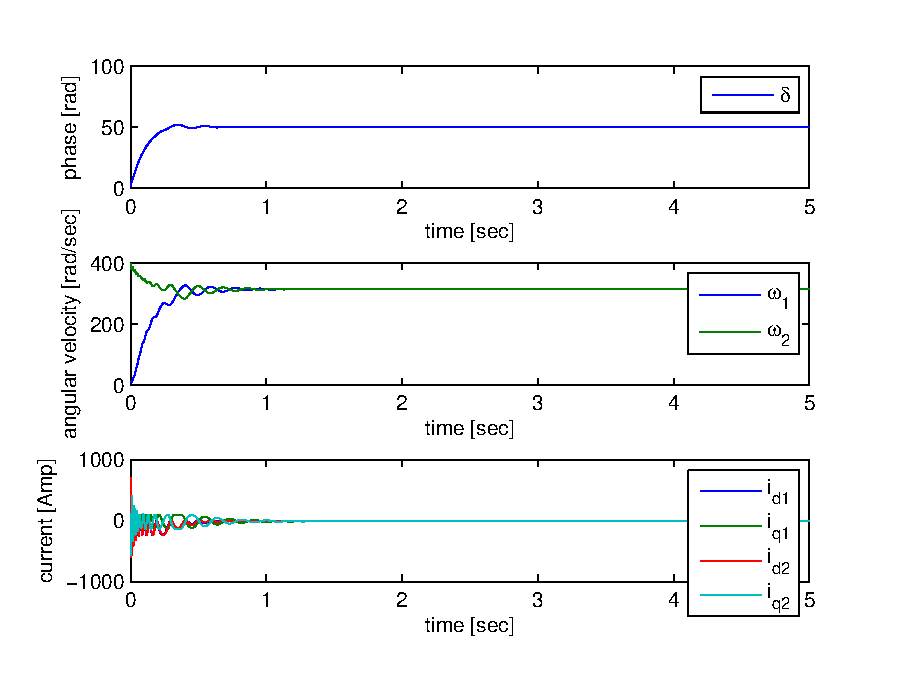
\includegraphics[scale=0.65]{5KWTICSGSimulation} \vspace{-8mm}
\caption{Simulations for TICSG system with 5KW SGs} 
\label{fig:5KWSGTICSGSimulation}
\end{figure}
%%%%%%%%%%**********%%%%%%%%%%**********%%%%%%%%%%**********%%%%%%%%%%

%%%%%%%%%%**********%%%%%%%%%%**********%%%%%%%%%%**********%%%%%%%%%%
\subsection{A stable but non globally stable equilibrium}

Note that Theorem \ref{theorem:TICSGSync} guarantee only local
stability, with $\Emscr$ contained in the region of attraction. 
Figure \ref{fig:InROATICSGSimulation} shows a simulation of a TICSG 
system similar to the previous one, but with smaller $L_s$, for an
initial state which is close enough to $\Emscr$, $\left[z_1(0)\ z_2(0)
\ \delta(0)\right]^\top=\left[40,\ -20,\ 70,\ 400,\ -20,\ 65,\ 0
\right]^\top$, such that the system stabilizes (in particular, the SGs
synchronize). 

Figure \ref{fig:OutROATICSGSimulation} shows another simulation for
the same system, with the initial state $\left[z_1(0)\ z_2(0) \
\delta(0) \right]^\top=\left[-400,\ -200,\ 10,\ 700,\ -20,\ 400,\
1.5708\right]^\top$. \m The simu\-lation indicates that this initial
state is outside the region of attraction, the SGs do not
synchronize. The parameters for the two simulations in this subsection
are $J=0.2$ {[}$kg\cdot m^{2}${]}, $D_{p}=1.7$ {[}$J\cdot sec${]}, $R_{s}=0.152$
{[}$\Omega]$, $R_{L}=18.862$ {[}$\Omega]$, $L_{s}=0.41$ {[}$mH${]},
$mi_{f}=1.05$ {[}$V\cdot sec]$, $T_{m}=543.2031$ {[}$N\cdot m${]}.

\vspace{-4mm}
%%%%%%%%%%**********%%%%%%%%%%**********%%%%%%%%%%**********%%%%%%%%%%
\begin{figure}[ht]
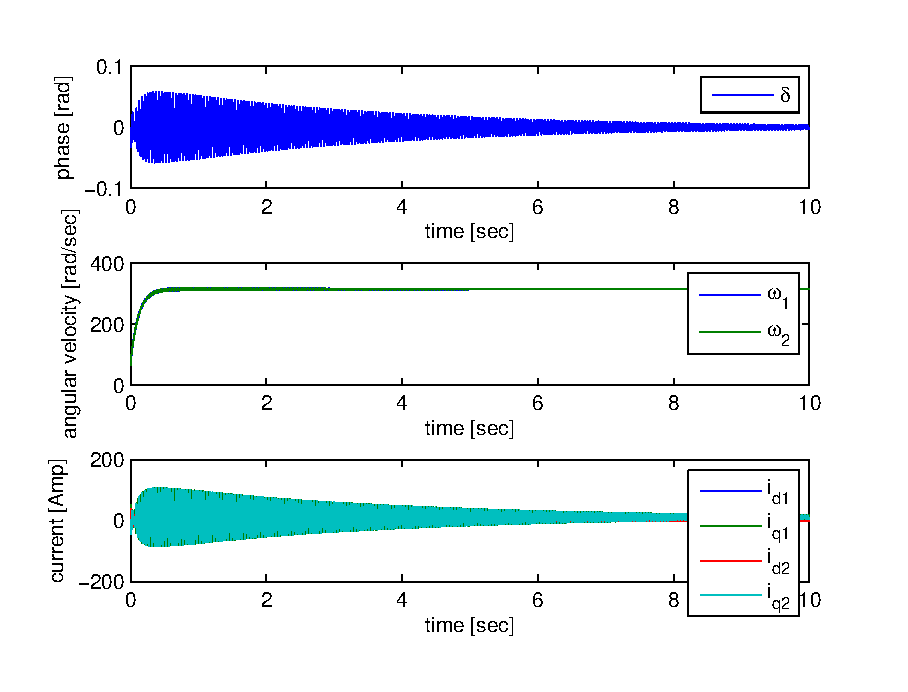
\includegraphics[scale=0.65]{InROATICSGSimulation}
\caption{Simulation for a TICSG system that satisfies the conditions
of Theorem \ref{theorem:TICSGSync}, with initial state inside the 
region of attraction of the stable equilibrium point.}
\label{fig:InROATICSGSimulation}
\end{figure}
%%%%%%%%%%**********%%%%%%%%%%**********%%%%%%%%%%**********%%%%%%%%%%

\vspace{-4mm}
%%%%%%%%%%**********%%%%%%%%%%**********%%%%%%%%%%**********%%%%%%%%%%
\begin{figure}[ht]
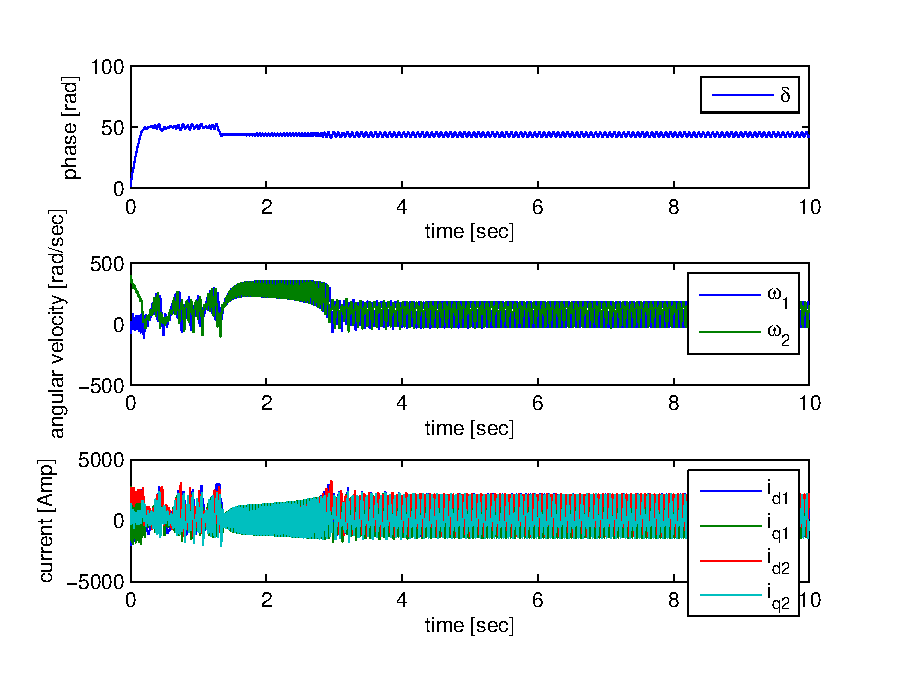
\includegraphics[scale=0.65]{OutROATICSGSimulation}

\caption{Simulation for a TICSG system which satisfy the conditions of
Theorem \ref{theorem:TICSGSync}, with initial state outside the region
of attraction of the stable equilibrium point.}
\label{fig:OutROATICSGSimulation}
\end{figure}
%%%%%%%%%%**********%%%%%%%%%%**********%%%%%%%%%%**********%%%%%%%%%%

%%%%%%%%%%**********%%%%%%%%%%**********%%%%%%%%%%**********%%%%%%%%%%
\subsection{Non stable $\mathscr{E}$ manifold}

%%%%%%%%%%**********%%%%%%%%%%**********%%%%%%%%%%**********%%%%%%%%%%
\begin{figure}[ht]
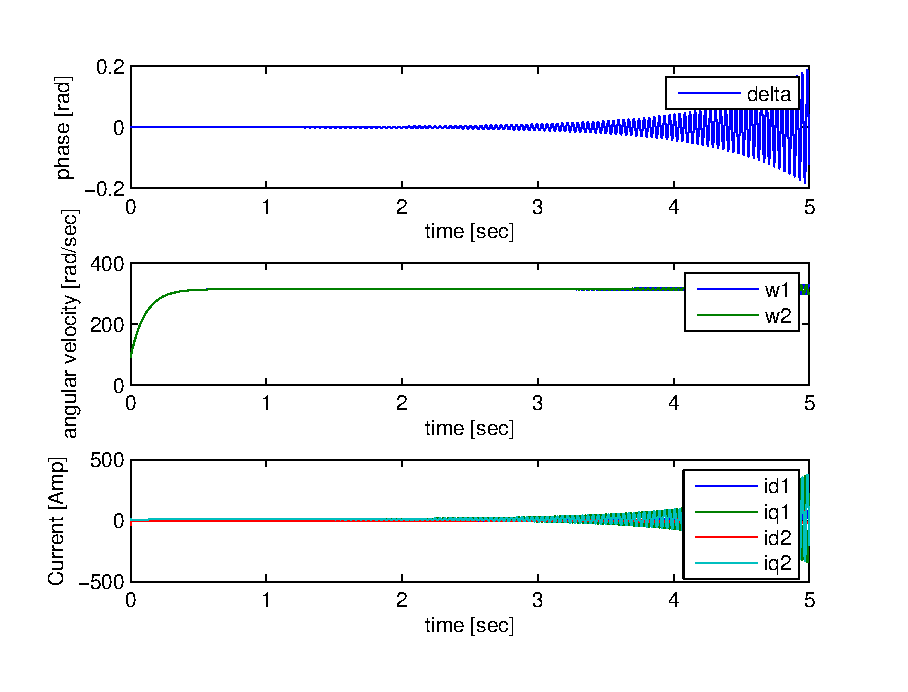
\includegraphics[scale=0.65]{NonStableTICSGSimulation}

\caption{A simulation example with unstable $\Emscr$ manifold}
\label{fig:NonStableTICSGSimulation}
\end{figure}
%%%%%%%%%%**********%%%%%%%%%%**********%%%%%%%%%%**********%%%%%%%%%%

Figure \ref{fig:NonStableTICSGSimulation}, shows an example where the
manifold $\mathscr{E}$ is not locally stable. Simulation of TICSG
system starting form the initial condition $\left[z_1(0)\ z_2(0) \
\delta(0) \right]^\top = \left[ -40, \ 20, \ 90, \ -40, \ 20, \ 90.01,
\ 0 \right]^\top$ do not synchronized. Note that condition
\eqref{eq:eLinearizationLimit} of Theorem \ref{theorem:TICSGSync} does
not hold. The parameters for this simulation are $J=0.2$
{[}$kg\cdot m^{2}${]}, $D_{p}=1.7$ {[}$J\cdot sec${]}, $R_{s}=0.152$
{[}$\Omega]$, $R_{L}=18.862$ {[}$\Omega]$, $L_{s}=0.35$ {[}$mH${]},
$mi_{f}=1.05$ {[}$V\cdot sec]$, $T_{m}=543.2031$ {[}$N\cdot m${]}.
%
%%%%%%%%%%%++++++++++%%%%%%%%%%++++++++++%%%%%%%%%%++++++++++%%%%%%%%%%

%%%%%%%%%%++++++++++%%%%%%%%%%++++++++++%%%%%%%%%%++++++++++%%%%%%%%%%
\section{Conclusions}

We have investigated a grid composed of a two identical SGs in
parallel and a resistive load. We have shown that this system has
equilibrium points only on the synchronization subspace or
anti-synchronization subspace. We have shown that there is exactly one
equilibrium point on the synchronization subspace, and this is stable
if $16 R_T D_p>L_s^2\left(\left(x_q^e\right)^2+\left(x_d^e\right)^2
\right)$. By a change of coordinates, we have rewritten the state as a
pair of vectors $(e,x)$ where $e$ is the difference between the states
of the two generators, and the system has the form 
\eqref{eq:systemForm}. If at the equilibrium point $(0,x^e)$,
$A=\frac{\partial F(e,x)}{\partial e}\left(0,x^e\right)$ is a Hurwitz
matrix, then the synchronization subspace $\mathscr{E}$ (which
consists of those states where $e=0$) is contained in the region of
attraction of the stable equilibrium point for the TICSG system. We
have shown by an example that, in general, this region of attraction
is not the whole state space.

%%%%%%%%%%++++++++++%%%%%%%%%%++++++++++%%%%%%%%%%++++++++++%%%%%%%%%%
\begin{thebibliography}{99}
 
\bibitem{AndrieuJayawardhanaPraly} V.~Andrieu, B.~Jayawardhana and
 L.~Praly, \m On the transverse exponential stability and its use in
 incremental stability, observer and synchronization. In {\em Proc. of
 the 52nd IEEE Conference on Decision and Control,} \m 2013.

\bibitem{CaTa:14} S.Y.~Caliskan and P.~Tabuada, \m
 Compositional transient stability analysis of multimachine 
 power networks, {\em IEEE Trans. Control of Network Systems}, 
 vol.~1, 2014, pp.~4-14.

\bibitem{DoBull:12} F. D{\"o}rfler and F. Bullo, \m 
 \emph{Synchronization and transient stability in power networks and
 nonuniform Kuramoto oscillators}.\hskip 1em plus 0.5em minus 
 0.4em\relax SIAM J. Control and Optim., vol.~50, 2012, 
 pp.~1616-1642.

\bibitem{Fitzgerald:03} A.E.~Fitzgerald, C.~Kingsley and S.D.~Umans,
 \m {\em Electric Machinery}, \m McGraw-Hill, New York, 2003.

\bibitem{GOBS:03}
 M.~Galaz, R.~Ortega, A.S.~Bazanella and A.M.~Stankovic, \m
 An energy-shaping approach to the design of excitation control
 of synchronous generators, {\em Automatica}, vol.~39, 2003,
 pp.~111-119.

\bibitem{GrSt2014} J.J.~Grainger and W.D.~Stevenson,
 {\em Power Systems Analysis}, \m McGraw-Hill, New York, 1994.
 
\bibitem{JayWeissBS:09}
 B.~Jayawardhana and G.~Weiss, \m State convergence of passive
 nonlinear systems with an $L^2$ input, {\em IEEE Trans. Automatic 
 Control}, 54 (2009), pp.~1723-1727.

\bibitem{Khalil} H.K.~Khalil, \m \emph{Nonlinear Systems} (third 
 edition), Prentice Hall, New Jersey, 2002.

\bibitem{Kundur} P.~Kundur, \emph{Power System Stability and Control}.
 \hskip 1em plus 0.5em minus 0.4em\relax McGraw-Hill, New York, 1994.

\bibitem{MaWe:15}
 Y.~Mandel and G.~Weiss, \m Adaptive internal model based
 suppression of torque ripple in brushless DC motor drives, {\em
 Systems Science \& Control Engineering}, vol.~5, 2015, pp.~162-176.

\bibitem{DePersiSchaft:16} P.~Monshizadeh, C.~De Persis,
 N.~Monshizadeh and A.~van der Schaft, \m Nonlinear Analysis
 of an improved swing equation, \m subm.~2016.

\bibitem{NaWe:14} V.~Natarajan and G.~Weiss, \m Almost global 
 asymptotic stability of a constant field current synchronous 
 machine connected to an infinite bus, {\em Proc. of the 53rd 
 IEEE Conf. on Decision and Control}, Los Angeles, CA, Dec. 2014, 
 pp.~3272-3279.

\bibitem{NaWe:15} V.~Natarajan and G.~Weiss, \m Almost global 
 asymptotic stability of a grid-connected synchronous generator,
 submitted in 2015.

\bibitem{Sastry} S.~Sastry, \m \emph{Nonlinear Systems}.
 Springer-Verlag, New York, 1999.

\bibitem{SauerPai1998} P.~W.~Sauer and M.~A.~Pai, \m {\em Power 
 Systems Dynamics and Stability}, Stipes Publishing, Champaign,
 IL, 1997.

\bibitem{SchovanecGilliam1999} L.~Schovanec and D.~Gilliam, \m ODE
 and PDE lecture notes. {\em The department to Mathematics and 
 Statistics at Texas Tech University. Available at
 \url{http://texas.math.ttu.edu/~gilliam/ttu/ode_pde_pdf/Ch4.pdf} }
 \m 1999.

\bibitem{PoDoBu:13} J.W.~Simpson-Porco, F.~D{\"o}rfler
 and F.~Bullo, \m Synchronization and power sharing for
 droop-controlled inverters in islanded microgrids, {\em 
 Automatica}, vol.~49, 2013, pp.~2603-2611.

\bibitem{Walker:94} J.H.~Walker, \m {\em Large Synchronous Machines: 
 Design, Manufacture and Operation}, \m Oxford University Press, 
 Oxford, 1981.

\bibitem{ZhWe:11} Q.-C.~Zhong and G.~Weiss, \m Synchronverters: 
 Inverters that mimic synchronous generators, {\em IEEE Trans. 
 Industr. Electronics}, vol.~58, 2011, pp.~1259-1267.

\end{thebibliography}
\end{document}
